\documentclass[table]{beamer}
\usepackage[utf8]{inputenc}
\usepackage{xcolor}
\usepackage{tcolorbox}
\usepackage{adjustbox}
\usepackage{multicol}
\usepackage{multirow}
\usepackage{eurosym}
\usepackage{amsmath}
\usepackage{ragged2e}
\usepackage[scaled]{helvet}
\usepackage{tikz}
\usepackage{eurosym}
\usetikzlibrary{spy,shapes,arrows,positioning,decorations.pathreplacing,matrix,calligraphy,calc}

\tikzset{hide on/.code={\only<#1>{\color{white}}}}
\definecolor{dark_green}{rgb}{0.0, 0.5, 0.0}

\pgfdeclarelayer{bg}    % declare background layer
\pgfsetlayers{bg,main}  % set the order of the layers (main is the standard layer)

\apptocmd{\frame}{}{\justifying}{}

\definecolor{iscal_color}{HTML}{641242} % ISCAL

\setbeamertemplate{footline}{
	\hspace{0.05\textwidth}
	\raisebox{3ex}{\insertshortauthor{}}\hfill
	\raisebox{3ex}{\insertframenumber{}/\inserttotalframenumber} \hfill
	{
\includegraphics[height=0.08\textheight]{../visual material/logo.png}}
	\hspace{0.05\textwidth}
}

\tikzset{
  invisible/.style={opacity=0},
  visible on/.style={alt={#1{}{invisible}}},
  alt/.code args={<#1>#2#3}{%
    \alt<#1>{\pgfkeysalso{#2}}{\pgfkeysalso{#3}} % \pgfkeysalso doesn't change the path
  },
}

\title{Microeconomia}
\subtitle{Capitulo 3A : Elasticidades e Interven\c c\~ao do Estado nos Mercados}
\author[]{}
\institute[ISCAL]{
\includegraphics[height=0.10\textheight]{../visual material/logo_eng_full.png}}
\date{Primavera 2020/2021}

\setbeamertemplate{navigation symbols}{}

\setbeamercolor{title}{fg = iscal_color}
\setbeamercolor{subtitle}{fg = iscal_color}
\setbeamercolor{frametitle}{fg = white, bg = iscal_color}

\hypersetup{linkcolor=iscal_color, colorlinks=true}

\AtBeginSection{\frame{\sectionpage}}
\renewcommand{\sectionname}{Parte}

\begin{document}

{
\setbeamertemplate{footline}{}
\begin{frame}
	\maketitle
\end{frame}
}

\begin{frame}{Conte\'udos}
  \tableofcontents
\end{frame}

\section{Elasticidade e elasticidade da Procura}
\begin{frame}
	\frametitle{A elasticidade como medida}
	\begin{itemize}
		\item A elasticidade \'e uma medida da varia\c c\~ao percentual de uma vari\'avel como resposta \`a varia\c c\~ao percentual da outra.
		\item Em \underline{termos discretos}, e considerando uma situa\c c\~ao inicial representada pelo ponto $(x_1,y_1)$ e uma situa\c c\~ao final representada pelo ponto $(x_2,y_2)$, a elasticidade de $Y$ em rela\c c\~ao a $X$ ser\'a calculada como \[\frac{\Delta\% \text{ em } Y}{\Delta\% \text{ em } X}=\frac{\frac{\Delta Y}{y_1}\times 100}{\frac{\Delta X}{x_1}\times 100}=\frac{\Delta Y}{\Delta X}\times\frac{x_1}{y_1}\]
	\end{itemize} 

	Onde $\Delta Z = z_2-z_1$.

\end{frame}

\begin{frame}
	\frametitle{A elasticidade como medida}
	\begin{itemize}
		\item Em \underline{termos cont\'inuos}, e conhecendo $Y=f(X)$, a elasticidade de $Y$ em rela\c c\~ao a $X$ ser\'a calculada como \(\frac{d Y}{d X} \frac{X}{Y}\)
		\item Vamos estudar as seguintes elasticidades:
	\end{itemize}
	\vspace{0.2cm}
	\begin{columns}
		\begin{column}{0.50\textwidth}
			{\color{blue} Elasticidades da procura}
			\begin{itemize}
				\item[$\varepsilon_{D}$] Pre\c co - direta da procura
				\item[$\varepsilon_{x,y}$] Pre\c co cruzada da procura
				\item[$\eta$] Rendimento da procura
			\end{itemize}
		\end{column}
		\begin{column}{0.47\textwidth}
			{\color{blue} Elasticidades da oferta}
			\begin{itemize}
				\item[$\varepsilon_{S}$] Pre\c co da Oferta
			\end{itemize}
			\vspace{1cm}
		\end{column}
	\end{columns}
\end{frame}

\begin{frame}
	\frametitle{A elasticidade como medida}
	As elasticidades da procura medem a varia\c c\~ao percentual da quantidade procurada quando h\'a uma varia\c c\~ao percentual de outra vari\'avel que a influencia. S\~ao o reflexo da sensibilidade do consumidor face a essa vari\'avel.
\end{frame}

\begin{frame}
	\frametitle{A elasticidade como medida}

		Elasticidade Pre\c co-Directa: \'e a varia\c c\~ao percentual da quantidade procurada quando h\'a uma varia\c c\~ao percentual do pre\c co do mesmo bem, ou seja: \[\varepsilon_D=\frac{\Delta\%Q_D}{\Delta\%P}=\frac{\frac{\Delta Q_D}{Q_D}}{\frac{\Delta P}{P}}={\color{blue}\frac{\Delta Q_D}{\Delta P}\frac{P}{Q_d}=\frac{dQ_D}{dP}\frac{P}{Q_d}}\]

		Mas $Q_D=a-bP$, assim $\frac{dQ_D}{dP}=-b$, assim em geral, $\varepsilon_D<0$

\end{frame}

\begin{frame}
	\frametitle{A elasticidade como medida}
	Classifica\c c\~ao da procura quanto \`a $\varepsilon_D$:
	\begin{itemize}
		\setlength\itemsep{0.5cm}
		\item $|\varepsilon_D|>1$ $\Rightarrow$ a procura \'e el\'astica
		\item $|\varepsilon_D|=1$ $\Rightarrow$ a procura tem elasticidade unit\'aria
		\item $|\varepsilon_D|<1$ $\Rightarrow$ a procura \'e inel\'astica ou r\'igida
	\end{itemize}

\end{frame}

\begin{frame}
	\frametitle{Elasticiade Pre\c co da Procura}

	$Q_D=100-5P$ para a forma linear $Q_D=a-b\times P$

	\begin{center}
		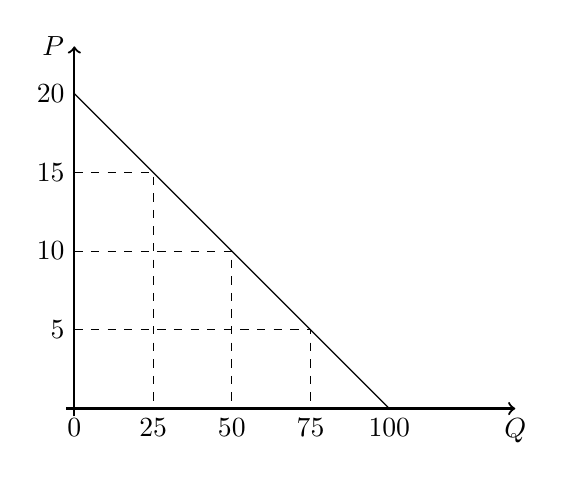
\begin{tikzpicture}[
			scale = 1,
			every node/.style = {scale = 1},
			declare function ={
				d(\x) = 4-\x;
			}
			]

			\draw[->,thick] (-0.1,0) -- (5.6,0)node[below]{$Q$};
			\draw[->,thick] (0,-0.1) -- (0,4.6)node[left]{$P$};

			\draw[domain=0:4,variable=\x] plot (\x,{d(\x)})node[below]{$100$};

			\foreach \n/\m in {5/75,10/50,15/25,20/0}{
				\draw[dashed](0,{\n/5})node[left]{$\n$} -- ({d(\n/5)},{\n/5}) -- ({d(\n/5)},0)node[below]{$\m$};
			}

		\end{tikzpicture}
		\par
		Qual a elasticidade pre\c co-directa na procura quando $P=15$? e $P=10$? e $P=5$?
	\end{center}

\end{frame}

\begin{frame}
	\frametitle{Elasticidade Pre\c co-Directa}
	\[\varepsilon_D=\frac{\Delta\% Q_D}{\Delta\% P}=\frac{\frac{\Delta Q_D}{q}}{\frac{\Delta P}{p}}=\frac{\Delta Q_D}{\Delta P}\frac{p}{q}\]
	No nosso caso:\[Q_D=100-5P\quad\Rightarrow\quad\Delta Q_D=-5\Delta P\] Logo \[\frac{\Delta Q_D}{\Delta P}=-5\]
\end{frame}

\begin{frame}
	\frametitle{Elasticidade Pre\c co-Directa}
	Quando $P=15$, $Q=25$, Logo:\[\varepsilon_D=\frac{\Delta \% Q_D}{\Delta \% P}=\frac{\frac{\Delta Q_D}{q}}{\frac{\Delta P}{p}}=\frac{\Delta Q_D}{\Delta P}\frac{p}{q}=-5\times\frac{15}{25}=-3\]
	Quando $P=15$, se o pre\c co aumentar 1\%, a quantidade procurada reduz-se 3\%.\par
	Como $|\varepsilon|>1$, diz-se que, neste ponto, a procura \'e \textbf{el\'astica}.
\end{frame}

\begin{frame}
	\frametitle{Elasticidade Pre\c co-Directa}
	Quando $P=5$, $Q=75$, Logo:\[\varepsilon_D=\frac{\Delta \% Q_D}{\Delta \% P}=\frac{\frac{\Delta Q_D}{q}}{\frac{\Delta P}{p}}=\frac{\Delta Q_D}{\Delta P}\frac{p}{q}=-5\times\frac{5}{75}=-0.33\]
	Quando $P=5$, se o pre\c co aumentar 1\%, a quantidade procurada reduz-se 0.33\%.\par
	Como $|\varepsilon|<1$, diz-se que, neste ponto, a procura \'e \textbf{inel\'astica}.
\end{frame}

\begin{frame}
	\frametitle{Elasticidade Pre\c co-Directa}
	Quando $P=10$, $Q=50$, Logo:\[\varepsilon_D=\frac{\Delta \% Q_D}{\Delta \% P}=\frac{\frac{\Delta Q_D}{q}}{\frac{\Delta P}{p}}=\frac{\Delta Q_D}{\Delta P}\frac{p}{q}=-5\times\frac{10}{50}=-1\]
	Quando $P=5$, se o pre\c co aumentar 1\%, a quantidade procurada reduz-se 1\%.\par
	Como $|\varepsilon|=1$, diz-se que, neste ponto, a procura tem elasticidade \textbf{unit\'aria}.
\end{frame}

\begin{frame}
	\frametitle{Elasticiade Pre\c co da Procura}

	$Q_D=100-5P$ para a forma linear $Q_D=a-b\times P$

	\begin{center}
		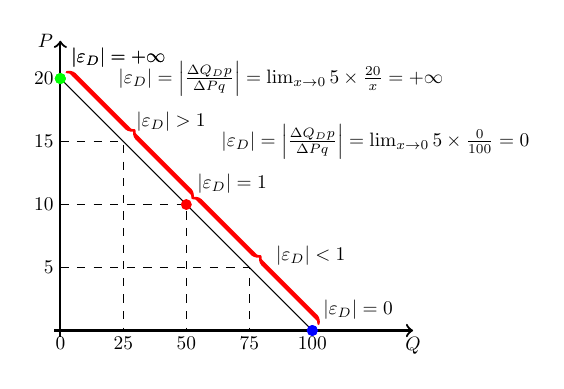
\begin{tikzpicture}[
			scale = 0.8,
			every node/.style = {scale = 0.7},
			declare function ={
				d(\x) = 4-\x;
			}
			]

			\draw[->,thick] (-0.1,0) -- (5.6,0)node[below]{$Q$};
			\draw[->,thick] (0,-0.1) -- (0,4.6)node[left]{$P$};

			\draw[domain=0:4,variable=\x] plot (\x,{d(\x)})node[below]{$100$};

			\onslide<1-4>{
				\foreach \n/\m in {5/75,10/50,15/25,20/0}{
					\draw[dashed](0,{\n/5})node[left]{$\n$} -- ({d(\n/5)},{\n/5}) -- ({d(\n/5)},0)node[below]{$\m$};
				}
			}

			\onslide<2->{
				\draw(2,2)node[circle,fill=red,inner sep=2,label=above right:{\(|\varepsilon_D|=1\)}]{};
			}

			\onslide<3-4>{
				\draw[pen colour={red},ultra thick,decorate,decoration={calligraphic brace},yshift=0.1cm,xshift=0.1cm] (2,2) -- (4,0) node[midway,xshift=1cm,yshift=0.1cm]{$|\varepsilon_D|<1$};
			}

			\onslide<4-4>{
				\draw[pen colour={red},ultra thick,decorate,decoration={calligraphic brace},yshift=0.1cm,xshift=0.1cm] (0,4) -- (2,2) node[midway,xshift=0.75cm,yshift=0.25cm]{$|\varepsilon_D|>1$};
			}

			\onslide<5-6>{
				\draw(0,4)node[circle,fill=green,inner sep=2]{};
			}

			\onslide<6>{
				\draw(3.5,4)node[]{$|\varepsilon_D|=\left|\frac{\Delta Q_D p}{\Delta P q}\right|=\lim_{x\rightarrow0}5\times\frac{20}{x}=+\infty$};
			}

			\onslide<7-8>{
				\draw(4,0)node[circle,fill=blue,inner sep=2]{};
				\draw(0,4)node[circle,fill=green,inner sep = 2,label=above right:{\(|\varepsilon_D|=+\infty\)}]{};
			}

			\onslide<8>{
				\draw(5,3)node[]{$|\varepsilon_D|=\left|\frac{\Delta Q_D p}{\Delta P q}\right|=\lim_{x\rightarrow0}5\times\frac{0}{100}=0$};
			}

			\onslide<9>{
				\draw(4,0)node[circle,fill=blue,inner sep=2,label=above right:{\(|\varepsilon_D|=0\)}]{};
				\draw(0,4)node[circle,fill=green,inner sep = 2,label=above right:{\(|\varepsilon_D|=+\infty\)}]{};
			}

		\end{tikzpicture}
	\end{center}
		\par
		Ao longo de uma procura linear, a elasticidade vai-se alterando. \onslide<5-8>{\color{green!80!black} Qual \'e a elasticidade no ponto verde?}\onslide<7-8>{\color{blue} e no ponto azul?}
\end{frame}

\begin{frame}
	\frametitle{Elasticidade Pre\c co-Directa}
	Quanto maior $|\varepsilon_D|$ mais o consumidor \'e sens\'ivel \`as varia\c c\~oes de pre\c co:
	\begin{itemize}
		\item Se \'e muito sens\'ivel, ent\~ao a procura \'e el\'astica e a quantidade reage de forma mais do que proporcional em rela\c c\~ao \`a varia\c c\~ao de pre\c co.
		\item Se \'e pouco sens\'ivel, ent\~ao a procura \'e inel\'astica e a quantidade reage de forma menos do que proporcional em rela\c c\~ao \`a varia\c c\~ao de pre\c co.
	\end{itemize}
\end{frame}

\begin{frame}
	\frametitle{Factores que influenciam a Elasticidade Pre\c co-Directa da Procura}
	\begin{itemize}
		\setlength{\itemsep}{0.3cm}
		\item Peso que a despesa de um bem tem no or\c camento para consumo
		\item Exist\^encia de mais bens substitutos
		\item Per\'iodo de tempo
	\end{itemize}
\end{frame}

\begin{frame}
	\frametitle{Elasticidade Pre\c co-Directa da Procura: Peso da despesa no or\c camento}
	Quanto maior o peso que a despesa de um bem tem no or\c camento para consumo, mais sens\'ivel ser\'a o consumidor \`as varia\c c\~oes de pre\c co, logo maior ser\'a a elasticidade.\pause
	\par
	\vspace{0.5cm}
	\'E natural, portanto,que as procuras lineares tenham uma zona el\'astica na parte superior, ou seja, quando os pre\c cos unit\'arios ultrapassam certo limiar...
\end{frame}
\begin{frame}
	\frametitle{Elasticidade Pre\c co-Directa da Procura: Exist\^encia de bens substitutos}
	A exist\^encia de mais bens substitutos, aumenta a elasticidade da procura de um bem:
	\begin{itemize}
		\item A elasticidade da procura de leite \'e inferior \`a elasticidade da procura de chantilly.
		\item \textbf{Consequ\^encia 1:} quanto mais espec\'ifica for a defini\c c\~ao de um bem, maior a elasticidade da procura.
		\item[*] A elasticidade da procura de leite \'e menor do que a elasticidade da procura de leite marca $X$.
		\item \textbf{Consequ\^encia 2:} bens essenciais com poucos substitutos t\^em procuras mais r\'igidas:
		\item[*] A elasticidade da procura de p\~ao \'e menor do que a elasticidade da procura de bolos.
	\end{itemize}
	
\end{frame}

\begin{frame}
	\frametitle{Elasticidade Pre\c co-Directa da Procura: Per\'iodo de tempo}
	Per\'iodo de tempo: a elasticidade tende a aumentar com o tempo decorrido, devido \`a possibilidade dos consumidores se conseguirem adaptar \`as varia\c c\~oes de pre\c co:
	\begin{itemize}
		\item A procura de curto-prazo de transporte em autocarro ter\'a uma elasticidade menor do que a procura de longo-prazo.
	\end{itemize}
\end{frame}

\begin{frame}
	\frametitle{Casos extremos}
	\begin{columns}
		\begin{column}{0.47\textwidth}
			\begin{center}
				\begin{tikzpicture}[
					scale = 0.7,
					every node/.style = {scale = 0.7},
					declare function ={
						d(\x) = 4-\x;
					}
					]

					\draw[->,thick] (-0.1,0) -- (5.6,0)node[below]{$Q$};
					\draw[->,thick] (0,-0.1) -- (0,4.6)node[left]{$P$};

					\draw(2,0)node[below]{$Q_0$} -- (2,4)node[midway,xshift=0.25cm]{$D$};

					\onslide<4->{
						\draw(3,1)node[right]{$|\varepsilon_D|=0$};
					}

				\end{tikzpicture}
			\end{center}
			{\scriptsize{
			\onslide<2->{\textbf{A quantidade procurada \'e independente do pre\c co} (para um intervalo de pre\c cos relevante)}\par
			\onslide<3->{(Ex: qualquer bem indispens\'avel \`a sobreviv\^encia e sem substitutos.. e.g.: medica\c c\~ao para doentes cr\'onicos)}
			}
			}
		\end{column}
		\begin{column}{0.47\textwidth}
			\begin{center}
				\begin{tikzpicture}[
					scale = 0.7,
					every node/.style = {scale = 0.7},
					declare function ={
						d(\x) = 4-\x;
					}
					]

					\draw[->,thick] (-0.1,0) -- (5.6,0)node[below]{$Q$};
					\draw[->,thick] (0,-0.1) -- (0,4.6)node[left]{$P$};

					\draw(0,2)node[left]{$P_0$} -- (4,2)node[midway,yshift=0.25cm]{$D$};

					\onslide<6->{
						\draw(3,1)node[right]{$|\varepsilon_D|=\infty$};
					}

				\end{tikzpicture}
			\end{center}
			
			\onslide<5->{
				\scriptsize{
				Os consumidores s\'o compram o bem ao pre\c co $P_0$. Se o pre\c co for maior, n\~ao compram e v\~ao procurar uma alternativa id\^entica mais barata.\par
				(Ex. Bens indiferenciados, homog\'eneos, i.e., com substitutos perfeitos)}
			}
		\end{column}
	\end{columns}
\end{frame}

\begin{frame}
	\frametitle{Casos interm\'edios}
	No mesmo intervalo de pre\c cos, as procuras podem ser mais ou menos el\'asticas. Depende do tipo de bem e dos factores que influenciam a elasticidade...\par

	obs: num intervalo de pre\c cos, a elasticidade calcula-se com refer\^encia ao ponto interm\'edio (elasticidade no arco). Verifique os c\'alculos em baixo... \[\varepsilon_D=\frac{\frac{\Delta Q}{\frac{Q_1+Q_2}{2}}}{\frac{\Delta P}{\frac{P_1+P_2}{2}}}\]
	\begin{center}
		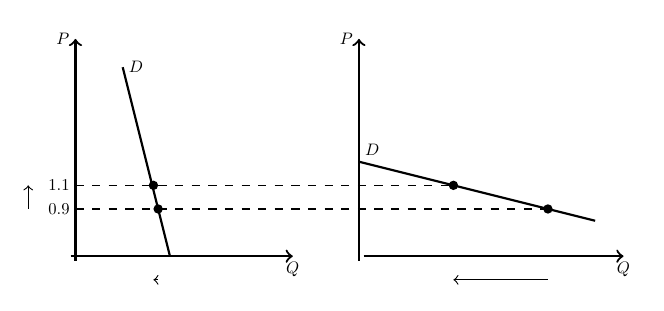
\begin{tikzpicture}[
			scale = 0.6,
			every node/.style={scale = 0.6}]

			\draw[->,thick] (-0.1,0) -- (4.6,0)node[below]{$Q$};
			\draw[->,thick] (0,-0.1) -- (0,4.6)node[left]{$P$};

			\draw[->,thick] (6.1,0) -- (11.6,0)node[below]{$Q$};
			\draw[->,thick] (6,-0.1) -- (6,4.6)node[left]{$P$};

			\draw[thick](1,4)node[right]{$D$}--(2,0);
			\draw[thick](6,2)node[above right]{$D$} -- (11,0.75);

			\draw[dashed](0,1.5)node[left]{$1.1$} -- (1.65,1.5) node[circle,fill,inner sep= 2pt]{} -- (8,1.5)node[circle,fill,inner sep=2pt]{};
			\draw[dashed](0,1)node[left]{$0.9$} -- (1.75,1) node[circle,fill,inner sep= 2pt]{} -- (10,1)node[circle,fill,inner sep=2pt]{};

			\onslide<2->{
				\draw[->](-1,1) -- (-1,1.5);
				\draw[->](1.75,-0.5) -- (1.65,-0.5);
				\draw[->](10,-0.5) -- (8,-0.5);
			}

		\end{tikzpicture}  
	\end{center}

\end{frame}

\begin{frame}
	\frametitle{Casos interm\'edios}
	Se no primeiro caso, $Q$ passa de 85 para 80, e no segundo caso $Q$ pasa de 205 para 95 obtemos o seguinte:
	\begin{align*}
		|\varepsilon_D|=\left|\frac{80-85}{1.1-0.9}\frac{\frac{1.1+0.9}{2}}{\frac{80+85}{2}}\right|=0.3
	\end{align*}

	Ou seja procura inel\'astica!

	Assim, para o segundo caso teremos:
	\begin{align*}
		|\varepsilon_D|=\left|\frac{95-205}{1.1-0.9}\frac{\frac{1.1+0.9}{2}}{\frac{205+95}{2}}\right|=3.7
	\end{align*}

	Ou seja procura el\'astica!
\end{frame}
\section{Elasticidade da Procura, despesa e outras elasticidades}
\begin{frame}
	\frametitle{Liguagem: interpretar e classificar}
	Se a elasticidade for, por exemplo, $|\varepsilon_D|=1.3$

	\begin{itemize}
		\setlength{\itemsep}{0.2cm}
		\item \textbf{\underline{Interpreta-se}} dizendo que a quantidade procurada reduz-se 1.3\% se o pre\c co aumentar 1\%, tudo o resto constante.
		\item \textbf{\underline{Classifica-se}} a procura como \underline{\emph{el\'astica}} no ponto onde o valor de $|\varepsilon_D|$ foi calculado.
	\end{itemize}
\end{frame}

\begin{frame}
	\frametitle{Elasticidade Pre\c co-Directa}
	A elasticidade pre\c co-directa da procura tem uma rela\c c\~ao directa com a varia\c c\~ao na despesa de consumo quando se altera um pre\c co.\par
	
	Vejamos o que acontece \`a despesa de consumo quando o pre\c co aumenta \euro 4 em dois cen\'arios diferentes, no exemplo seguinte:
	\begin{itemize}
		\item quando o pre\c co inicialmente \'e \euro 12
		\item quando o pre\c co inicialmente \'e \euro 4
	\end{itemize}
\end{frame}

\begin{frame}
	\frametitle{Elasticidade da Procura}
	$Q_D=100-5P$
	\begin{center}
		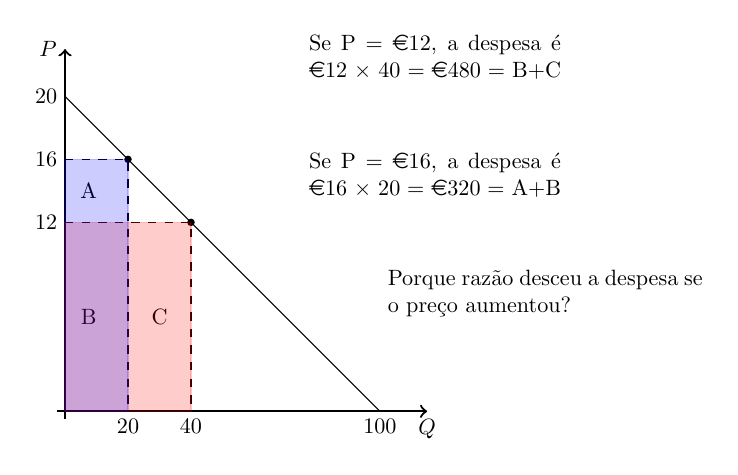
\begin{tikzpicture}[
			scale = 1,
			every node/.style = {scale = 0.8},
			declare function = {d(\x)=4-\x;}
			]

			\draw[->,thick] (-0.1,0) -- (4.6,0)node[below]{$Q$};
			\draw[->,thick] (0,-0.1) -- (0,4.6)node[left]{$P$};

			\draw[domain=0:4,variable=\x] plot (\x,{d(\x)}) node[below]{100};
			\draw(0,{d(0)}) node[left]{20};

			\onslide<2->{
				\draw[dashed](0,2.4)node[left]{12} -- (1.6,2.4)node[circle,fill,inner sep=1.2pt]{} -- (1.6,0)node[below]{40};
				\draw[dashed](0,3.2)node[left]{16} -- (0.8,3.2)node[circle,fill,inner sep=1.2pt]{} -- (0.8,0)node[below]{20};
			}


			\onslide<3->{
				\draw(0.3,2.8)node[]{A};
				\draw(0.3,1.2)node[]{B};
				\draw(1.2,1.2)node[]{C};
			}

			\onslide<4->{
				\draw(3,4.5)node[right]{\parbox{4cm}{Se P = \euro 12, a despesa \'e \euro 12 $\times$ 40 = \euro 480 = B+C}};
			}

			\onslide<5>{
				\draw[opacity=0.2,red,fill] (0,0)--(1.6,0)--(1.6,2.4)--(0,2.4)--(0,0);
			}

			\onslide<6->{
				\draw(3,3)node[right]{\parbox{4cm}{Se P = \euro 16, a despesa \'e \euro 16 $\times$ 20 = \euro 320 = A+B}};	
			}

			\onslide<7>{
				\draw[opacity=0.2,blue,fill] (0,0)--(0.8,0)--(0.8,3.2)--(0,3.2)--(0,0);
			}

			\onslide<8->{
				\draw(4,1.5)node[right]{\parbox{5cm}{Porque raz\~ao desceu a despesa se o pre\c co aumentou?}};	
			}

		\end{tikzpicture}
	\end{center}
\end{frame}


\begin{frame}
	\frametitle{Elasticidade da Procura}
	$Q_D=100-5P$
	\begin{center}
		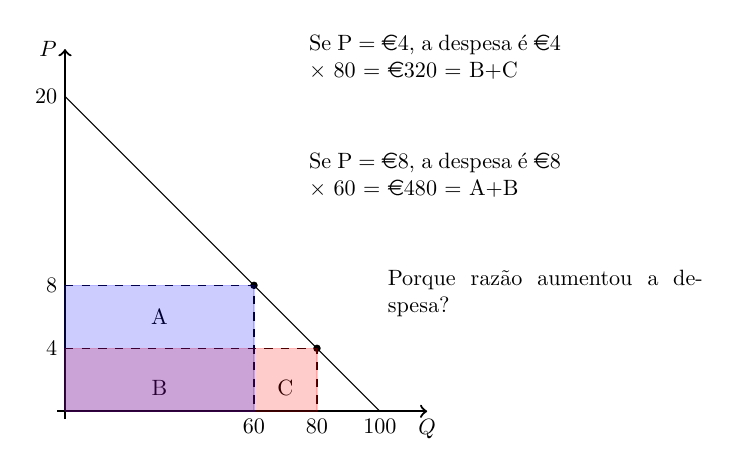
\begin{tikzpicture}[
			scale = 1,
			every node/.style = {scale = 0.8},
			declare function = {d(\x)=4-\x;}
			]

			\draw[->,thick] (-0.1,0) -- (4.6,0)node[below]{$Q$};
			\draw[->,thick] (0,-0.1) -- (0,4.6)node[left]{$P$};

			\draw[domain=0:4,variable=\x] plot (\x,{d(\x)}) node[below]{100};
			\draw(0,{d(0)}) node[left]{20};

			\onslide<2->{
				\draw[dashed](0,0.8)node[left]{4} -- (3.2,0.8)node[circle,fill,inner sep=1.2pt]{} -- (3.2,0)node[below]{80};
				\draw[dashed](0,1.6)node[left]{8} -- (2.4,1.6)node[circle,fill,inner sep=1.2pt]{} -- (2.4,0)node[below]{60};
			}


			\onslide<3->{
				\draw(1.2,1.2)node[]{A};
				\draw(1.2,0.3)node[]{B};
				\draw(2.8,0.3)node[]{C};
			}

			\onslide<4->{
				\draw(3,4.5)node[right]{\parbox{4cm}{Se P = \euro 4, a despesa \'e \euro 4 $\times$ 80 = \euro 320 = B+C}};
			}

			\onslide<5>{
				\draw[opacity=0.2,red,fill] (0,0)--(3.2,0)--(3.2,0.8)--(0,0.8)--(0,0);
			}

			\onslide<6->{
				\draw(3,3)node[right]{\parbox{4cm}{Se P = \euro 8, a despesa \'e \euro 8 $\times$ 60 = \euro 480 = A+B}};	
			}

			\onslide<7>{
				\draw[opacity=0.2,blue,fill] (0,0)--(2.4,0)--(2.4,1.6)--(0,1.6)--(0,0);
			}

			\onslide<8->{
				\draw(4,1.5)node[right]{\parbox{5cm}{Porque raz\~ao aumentou a despesa?}};	
			}

		\end{tikzpicture}
	\end{center}
\end{frame}

\begin{frame}
	\frametitle{Elasticidade e Despesa de Consumo}
	\[Despesa_0=P_0\times Q_0\]
	Seja $\Delta P$ a varia\c c\~ao no pre\c co e $\Delta Q$ a correspondente varia\c c\~ao na quantidade procurada. O valor da despesa total ap\'os a varia\c c\~ao do pre\c co ser\'a
	\[Despesa_1 = \overbrace{(P_0+\Delta P_0)}^{P_1}\times\overbrace{(Q_0+\Delta Q_0)}^{Q_1}\]
	\[=P_0\times Q_0 + P_0\times \Delta Q + \Delta P \times Q_0 + \Delta P \times \Delta Q\]
	Pelo que $\Delta Despesa=Despesa_1-Despesa_0$\[\Delta Despesa =P_0\times \Delta Q + \Delta P \times Q_0 + \Delta P \times \Delta Q\]
\end{frame}

\begin{frame}
	\frametitle{Elasticidade e Despesa de Consumo}
	Notar que se $\Delta P$ \'e pequeno, $\Delta Q$ tamb\'em hai de ser relativamente pequeno (em compara\c c\~ao \`a $Q$),  pelo que $\Delta P\times\Delta Q$ \'e ser\'a muito pequeno, assim podemos dizer que:\[\Delta Despesa \approx P_0\times \Delta Q + \Delta P \times Q_0\]
	Podemos identificar estes dois termos como:

	\begin{itemize}
			\item $\Delta P \times Q_0$ Efeito pre\c co (\'area A do gr\'afico)
			\item $P_0\times \Delta Q$ Efeito quantidade (\'area C do gr\'afico)
	\end{itemize}
\end{frame}

\begin{frame}
\frametitle{Elasticidade e Despesa de Consumo}

	Se a despesa aumenta:

	\begin{align*}
		P_0\times \Delta Q + \Delta P \times Q_0>0 &\Leftrightarrow P_0\times \Delta Q > -\Delta P \times Q_0 \\
		\Leftrightarrow \frac{P\Delta Q}{Q\Delta P}>-1&\Leftrightarrow \frac{\Delta Q}{\Delta P}\frac{P_0}{Q_0}>-1\\ |\varepsilon_D|&<1
	\end{align*}
\end{frame}

\begin{frame}
	\frametitle{Elasticidade e Despesa}
	Ent\~ao:
	\begin{itemize}
		\setlength{\itemsep}{0.5cm}
		\item Numa zona em que a procura \'e el\'astica, $|\varepsilon_D|>1$ um aumento de pre\c co significa uma redu\c c\~ao da despesa (predomina o efeito da redu\c c\~ao da quantidade)
		\item Numa zona em que a procura \'e r\'igida, $|\varepsilon_D|<1$ um aumento de pre\c co significa um aumento da despesa (predomina o efeito do aumento do pre\c co.)
	\end{itemize}
\end{frame}

\begin{frame}
	\frametitle{Elasticidade da Procura}
	$Q_D=100-5P$
	\begin{center}
		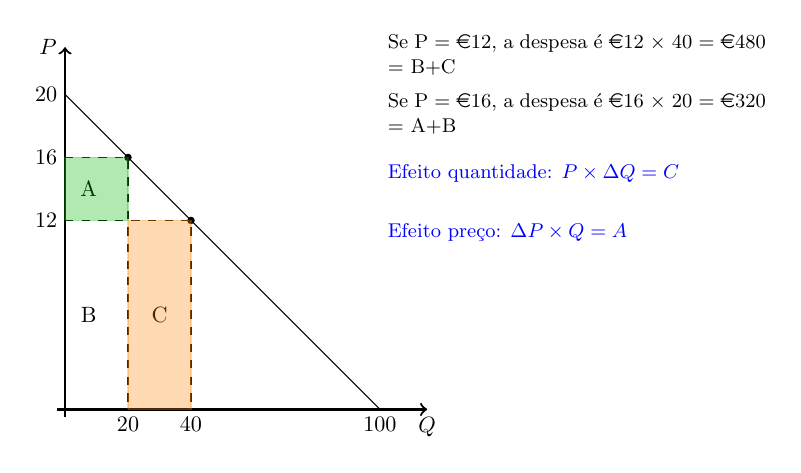
\begin{tikzpicture}[
			scale = 1,
			every node/.style = {scale = 0.8},
			declare function = {d(\x)=4-\x;}
			]

			\draw[->,thick] (-0.1,0) -- (4.6,0)node[below]{$Q$};
			\draw[->,thick] (0,-0.1) -- (0,4.6)node[left]{$P$};

			\draw[domain=0:4,variable=\x] plot (\x,{d(\x)}) node[below]{100};
			\draw(0,{d(0)}) node[left]{20};

			\draw[dashed](0,2.4)node[left]{12} -- (1.6,2.4)node[circle,fill,inner sep=1.2pt]{} -- (1.6,0)node[below]{40};
			\draw[dashed](0,3.2)node[left]{16} -- (0.8,3.2)node[circle,fill,inner sep=1.2pt]{} -- (0.8,0)node[below]{20};

			\draw(0.3,2.8)node[]{A};
			\draw(0.3,1.2)node[]{B};
			\draw(1.2,1.2)node[]{C};

			\draw(4,4.5)node[right]{\parbox{6cm}{\small Se P = \euro 12, a despesa \'e \euro 12 $\times$ 40 = \euro 480 = B+C}};
			\draw(4,3.75)node[right]{\parbox{6cm}{\small Se P = \euro 16, a despesa \'e \euro 16 $\times$ 20 = \euro 320 = A+B}};	

			\onslide<2->{
				\draw(4,3)node[right]{\color{blue}\parbox{6cm}{\small Efeito quantidade: $P\times\Delta Q=C$}};	
			}

			\onslide<3->{
				\draw[opacity=0.3,orange,fill] (0.8,0)--(1.6,0)--(1.6,2.4)--(0.8,2.4)--(0.8,0);
			}

			\onslide<4->{
				\draw(4,2.25)node[right]{\color{blue}\parbox{6cm}{\small Efeito pre\c co: $\Delta P\times Q=A$}};	
			}

			\onslide<5->{
				\draw[opacity=0.3,green!70!black,fill] (0,2.4)--(0.8,2.4)--(0.8,3.2)--(0,3.2)--(0,2.4);
			}

		\end{tikzpicture}
	\end{center}
\end{frame}

\begin{frame}
	\frametitle{Elasticidade da Procura}
	$Q_D=100-5P$
	\begin{center}
		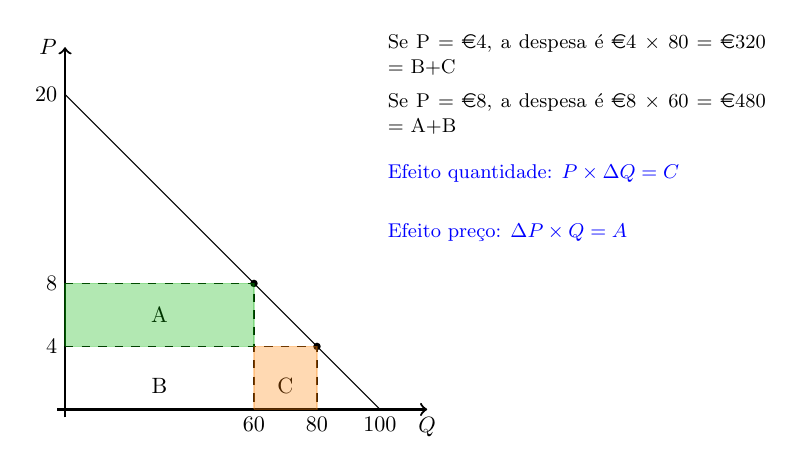
\begin{tikzpicture}[
			scale = 1,
			every node/.style = {scale = 0.8},
			declare function = {d(\x)=4-\x;}
			]

			\draw[->,thick] (-0.1,0) -- (4.6,0)node[below]{$Q$};
			\draw[->,thick] (0,-0.1) -- (0,4.6)node[left]{$P$};

			\draw[domain=0:4,variable=\x] plot (\x,{d(\x)}) node[below]{100};
			\draw(0,{d(0)}) node[left]{20};

			\draw[dashed](0,0.8)node[left]{4} -- (3.2,0.8)node[circle,fill,inner sep=1.2pt]{} -- (3.2,0)node[below]{80};
			\draw[dashed](0,1.6)node[left]{8} -- (2.4,1.6)node[circle,fill,inner sep=1.2pt]{} -- (2.4,0)node[below]{60};

			\draw(1.2,1.2)node[]{A};
			\draw(1.2,0.3)node[]{B};
			\draw(2.8,0.3)node[]{C};

			\draw(4,4.5)node[right]{\parbox{6cm}{\small Se P = \euro 4, a despesa \'e \euro 4 $\times$ 80 = \euro 320 = B+C}};
			\draw(4,3.75)node[right]{\parbox{6cm}{\small Se P = \euro 8, a despesa \'e \euro 8 $\times$ 60 = \euro 480 = A+B}};	

			\onslide<2->{
				\draw(4,3)node[right]{\color{blue}\parbox{6cm}{\small Efeito quantidade: $P\times\Delta Q=C$}};	
			}

			\onslide<3->{
				\draw[opacity=0.3,orange,fill] (2.4,0)--(3.2,0)--(3.2,0.8)--(2.4,0.8)--(2.4,0);
			}

			\onslide<4->{
				\draw(4,2.25)node[right]{\color{blue}\parbox{6cm}{\small Efeito pre\c co: $\Delta P\times Q=A$}};	
			}

			\onslide<5->{
				\draw[opacity=0.3,green!70!black,fill] (0,0.8)--(2.4,0.8)--(2.4,1.6)--(0,1.6)--(0,0.8);
			}

		\end{tikzpicture}
	\end{center}
\end{frame}

\begin{frame}
	\frametitle{Elasticidade da Procura e Despesa:$Q_D=100-5P$}

	\begin{columns}
		\begin{column}{0.6\textwidth}
			\begin{center}
				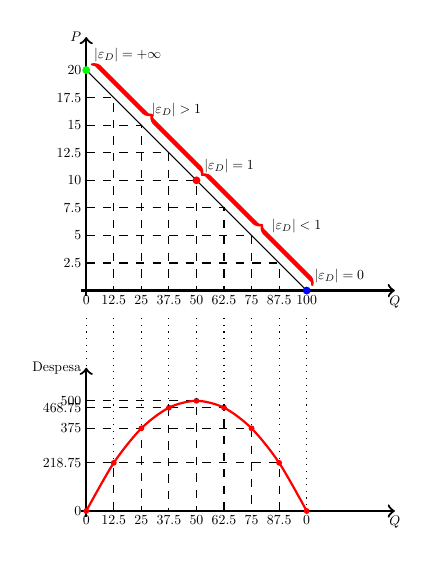
\begin{tikzpicture}[
					scale = 0.7,
					every node/.style = {scale = 0.5},
					declare function ={
						d(\x) = 4-\x;
					}
					]

					\draw[->,thick] (-0.1,0) -- (5.6,0)node[below]{$Q$};
					\draw[->,thick] (0,-0.1) -- (0,4.6)node[left]{$P$};

					\draw[domain=0:4,variable=\x] plot (\x,{d(\x)})node[below]{$100$};

					\foreach \n/\m in {2.5/87.5,5/75,7.5/62.5,10/50,12.5/37.5,15/25,17.5/12.5,20/0}{
						\draw[dashed](0,{\n/5})node[left]{$\n$} -- ({d(\n/5)},{\n/5}) -- ({d(\n/5)},0)node[below]{$\m$};
					}

					\draw(2,2)node[circle,fill=red,inner sep=2,label=above right:{\(|\varepsilon_D|=1\)}]{};
					\draw[pen colour={red},ultra thick,decorate,decoration={calligraphic brace},yshift=0.1cm,xshift=0.1cm] (2,2) -- (4,0) node[midway,xshift=1cm,yshift=0.1cm]{$|\varepsilon_D|<1$};
					\draw[pen colour={red},ultra thick,decorate,decoration={calligraphic brace},yshift=0.1cm,xshift=0.1cm] (0,4) -- (2,2) node[midway,xshift=0.75cm,yshift=0.25cm]{$|\varepsilon_D|>1$};

					\draw(4,0)node[circle,fill=blue,inner sep=2,label=above right:{\(|\varepsilon_D|=0\)}]{};
					\draw(0,4)node[circle,fill=green,inner sep = 2,label=above right:{\(|\varepsilon_D|=+\infty\)}]{};

					\onslide<2->{

					\draw[->,thick] (-0.1,-4) -- (5.6,-4)node[below]{$Q$};
					\draw[->,thick] (0,-4.1) -- (0,{4.6-6})node[left]{Despesa};

					}

					\onslide<3->{
						\foreach \n/\m/\k/\a in {0/0//a,2.5/87.5/218.75/b,5/75/375/c,7.5/62.5/468.75/d,10/50/500/e,12.5/37.5//f,15/25//g,17.5/12.5//h,20/0/0/i}{

							\draw[dashed](0,{(\n*d(\n/5))/10-4})node[left]{$\k$} -- ({d(\n/5)},{(\n*d(\n/5))/10-4})node[circle,fill,inner sep=1.5,red]{} -- ({d(\n/5)},-4)node[below]{$\m$};
							\draw[dotted]({d(\n/5)},-0.5) -- ({d(\n/5)},{(\n*d(\n/5))/10-4});

							\coordinate (\a) at ({d(\n/5)},{(\n*d(\n/5))/10-4});
						}
					}
					
					\onslide<4>{
						\draw[red,thick] plot [smooth] coordinates {(a) (b) (c) (d) (e) (f) (g) (h) (i)};
					}


				\end{tikzpicture}
			\end{center}
		\end{column}
		\begin{column}{0.375\textwidth}
			{\centering
			\footnotesize
			\begin{tabular}{ccc}
				$P$ & $Q_D$ & $P\times Q_D$\\\hline
				0 & 100 & 0 \\
				2.5 & 87.5 & 218.75 \\
				5 & 75 & 375 \\
				7.5 & 62.5 & 468.75 \\
				10 & 50 & 500 \\
				12.5 & 37.5 & 468.75 \\
				15 & 25 & 375 \\
				17.5 & 12.5 & 218.75 \\
				20 & 0 & 0
			\end{tabular}
		}
		\end{column}
	\end{columns}
\end{frame}

\begin{frame}
	\frametitle{Elasticidade e Despesa de Consumo}
	\begin{columns}
		\begin{column}{0.47\textwidth}
			Generalizando os Resultados:
			\begin{align*}
				Despesa&=RT=P\times Q\\
				P&=\frac{a}{b}-\frac{1}{b}Q\\
				\onslide<2->{
				RT&=\left(\frac{a}{b}-\frac{1}{b}Q\right)\times Q\\
				&=\frac{a}{b}Q-\frac{1}{b}Q^2\\
				}
				\onslide<3->{
				Rmg&=RT'=\frac{a}{b}-\frac{2}{b}Q\\
				Rmg&=0\Leftrightarrow Q=\frac{a}{2}
				}
			\end{align*}
		\end{column}
		\begin{column}{0.47\textwidth}
			\begin{center}
				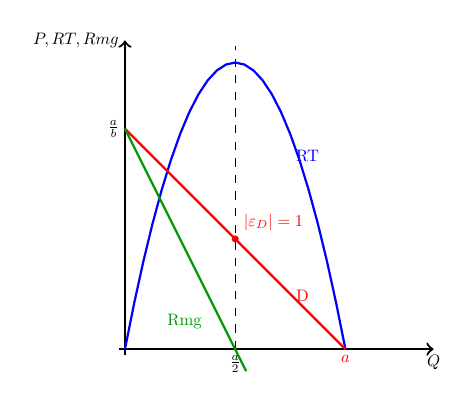
\begin{tikzpicture}[
					scale = 0.7,
					every node/.style = {scale = 0.6},
					declare function = {
						d(\x)=4-\x;
						rt(\x) = 1.3*(4-(\x-2)^2);
						rm(\x) = 4-(2)*\x;
					}]

					\onslide<4->{
						\draw[->,thick] (-0.1,0) -- (5.6,0)node[below]{$Q$};
						\draw[->,thick] (0,-0.1) -- (0,5.6)node[left]{$P,RT,Rmg$};
					}
					
					\onslide<5->{
						\draw[dashed] (2,0)node[below]{$\frac{a}{2}$} -- (2,5.5);
					}

					\onslide<6->{
						\draw[blue,thick,domain=0:4,variable=\x] plot (\x,{rt(\x)});
						\draw[blue] (3,3.5)node[right]{RT};
					}

					\onslide<7->{
						\draw[red,thick,domain=0:4,variable=\x] plot (\x,{d(\x)}) node[below]{$a$};
						\draw[red] (3,0.75)node[above right]{D};	
						\draw[red] (2,2)node[circle,fill,inner sep=1.5,label=above right:{\(|\varepsilon_D|=1\)}]{};
					}

					\onslide<8->{
						\draw[green!60!black,thick,domain=0:2.2,variable=\x] plot (\x,{rm(\x)});
						\draw[green!60!black] (1.5,0.5)node[left]{Rmg};
						\draw(0,{rm(0)}) node[left]{$\frac{a}{b}$};
					}

				\end{tikzpicture}
			\end{center}
		\end{column}
	\end{columns}
\end{frame}

\begin{frame}
	\frametitle{Elasticidade e Despesa de Consumo}
	Formalizando a rela\c c\~ao da receita marginal com a $|\varepsilon_D|$... \par
	Repare-se que $Rmg=\frac{\Delta RT}{\Delta Q}$ \[\Delta RT = \Delta P \times Q + P \Delta Q\] Donde,
	\[Rmg = \frac{\Delta Q\times P + P \times \Delta Q}{\Delta Q} = \frac{\Delta P \times Q}{\Delta Q}+P=P\times\left(\frac{\Delta P\times Q}{\Delta Q\times P}+1\right)=\]
	\[=P\times\left(1+\frac{1}{\varepsilon_D}\right)=P\times\left(1-\frac{1}{|\varepsilon_D|}\right)\]
	Voltaremos a este resultado no cap. 4 (monop\'olio)
\end{frame}

\begin{frame}
	\frametitle{Outras Elasticidades da Procura}
	\begin{itemize}
		\item Elasticidade procura-pre\c co cruzada \[\varepsilon_{x,y}=\frac{\Delta\%Q_x}{\Delta\%P_y}=\frac{\frac{\Delta Q_x}{q_x}}{\frac{\Delta P_y}{P_y}}=\frac{\Delta Q_x}{q_x}\frac{P_y}{\Delta P_y}=\frac{\Delta Q_x}{\Delta P_y}\frac{P_y}{q_x}\]
		\onslide<2->{
		\begin{itemize}
			\item $\varepsilon_{x,y}<0$ caso $X$ e $Y$ sejam bens complementares
			\item $\varepsilon_{x,y}>0$ caso $X$ e $Y$ sejam bens substitutos
			\item $\varepsilon_{x,y}=0$ caso $X$ e $Y$ sejam bens independentes
		\end{itemize}
		}
	\end{itemize}
	\onslide<3->{
	\'E uma ferramenta especialmente importante para determinar os bens que fazem parte do mesmo mercado... quanto mais elevada for $\varepsilon_{x,y}$ maior a influ\^encia m\'utua dos pre\c cos dos bens e, portanto, far\~ao parte do mesmo mercado: iogurtes mimosa e iogurtes danone far\~ao parte do mesmo mercado... mas iogurtes mimosa e ervilhas iglo ser\~ao bens de mercados diferentes, pois nesse caso $\varepsilon_{x,y}=0$}
\end{frame}

\begin{frame}
	\frametitle{Outras Elasticidades da Procura}
	\begin{itemize}
		\item Elasticidade procura-rendimento \[\eta=\frac{\Delta \% Q}{\Delta\% W}=\frac{\frac{\Delta Q}{q}}{\frac{\Delta W}{w}}=\frac{\Delta Q}{\Delta W}\frac{w}{q}\]
	\end{itemize}
	\begin{itemize}
		\item $\eta<0$ para bens inferiores
		\item $\eta>0$ para bens normais
		\onslide<2->{\item $\eta>1$ para bens de luxo}
	\end{itemize}
	Mede a sensibilidade do consumidor face a varia\c c\~oes de rendimento dispon\'ivel para o consumo de um determinado bem.
\end{frame}

\begin{frame}
	\frametitle{Elasticidade Pre\c co da Oferta}
	Calcula-se exactamente da mesma forma do que a elasticidade pre\c co-directa da procura, mas ao longo da curva da oferta...
	\[\varepsilon_s=\frac{\Delta\%Q_S}{\Delta\%P}=\frac{\frac{\Delta Q_S}{Q_S}}{\frac{\Delta P}{P}}=\frac{\Delta Q_S}{\Delta P}\frac{P}{Q_S}\]
	A elasticidade pre\c co da oferta ser\'a \underline{\textbf{sempre positiva}}.

\end{frame}

\begin{frame}
	\frametitle{Elasticidade Pre\c co da Oferta}
	Classifica\c c\~ao da ofeta quanto \`a $\varepsilon_S$
	\begin{itemize}
		\item $\varepsilon_S>1$ $\Rightarrow$ a oferta \'e el\'astica
		\item $\varepsilon_S=1$ $\Rightarrow$ a oferta tem elasticidade unit\'aria
		\item $\varepsilon_S<1$ $\Rightarrow$ a oferta \'e inel\'astica
	\end{itemize}
\end{frame}



\begin{frame}
	\frametitle{Casos extremos}
	\begin{columns}
		\begin{column}{0.47\textwidth}
			\begin{center}
				\begin{tikzpicture}[
					scale = 0.7,
					every node/.style = {scale = 0.7},
					declare function ={
						d(\x) = 4-\x;
					}
					]

					\draw[->,thick] (-0.1,0) -- (5.6,0)node[below]{$Q$};
					\draw[->,thick] (0,-0.1) -- (0,4.6)node[left]{$P$};

					\draw(2,0)node[below]{$Q_0$} -- (2,4)node[midway,xshift=0.25cm]{$S$};

					\onslide<4->{
						\draw(3,1)node[right]{$|\varepsilon_S|=0$};
					}

				\end{tikzpicture}
			\end{center}
			{\scriptsize{
			\onslide<2->{\textbf{A quantidade oferecida \'e independente do pre\c co} (para um intervalo de pre\c cos relevante)}\par
			\onslide<3->{(Ex: qualquer bem para o qual n\~ao seja poss\'ivel aumentar a produ\c c\~ao por aus\^encia de fatores produtivos, e.g.; obras de arte, pe\c cas \'unicas.)}
			}
			}
		\end{column}
		\begin{column}{0.47\textwidth}
			\begin{center}
				\begin{tikzpicture}[
					scale = 0.7,
					every node/.style = {scale = 0.7},
					declare function ={
						d(\x) = 4-\x;
					}
					]

					\draw[->,thick] (-0.1,0) -- (5.6,0)node[below]{$Q$};
					\draw[->,thick] (0,-0.1) -- (0,4.6)node[left]{$P$};

					\draw(0,2)node[left]{$P_0$} -- (4,2)node[midway,yshift=0.25cm]{$S$};

					\onslide<6->{
						\draw(3,1)node[right]{$|\varepsilon_S|=\infty$};
					}

				\end{tikzpicture}
			\end{center}
			
			\onslide<5->{
				\scriptsize{
				Para $P=P_0$ os produtores oferecer\~ao qualquer quantidade... uma expans\~ao da procura n\~ao provocar\'a efeitos inflacionistas... (guardar a informa\c c\~ao para quando se estudar os modelos Keynesianos em Macroeconomia)}
			}
		\end{column}
	\end{columns}
\end{frame}

\begin{frame}
	\frametitle{Factores que influenciam a elasticidade pre\c co da oferta}
	\begin{itemize}
		\item Disponibilidade dos fatores de produ\c c\~ao (incluindo substituibilidade e mobilidade):
		\begin{itemize}
			\item Um quadro de Rembrandt tem uma oferta totalmente, r\'igida, mas a oferta de p\~ao tem uma elasticidade bastante elevada
			\item A oferta de Pizzas ser\'a mais el\'astica do que a oferta de morangos (principalmente se for fora da esta\c c\~ao)
		\end{itemize}
		\item Capacidade produtiva:
		\begin{itemize}
			\item A oferta de transporte a\'ereo \'e inifnitamente el\'astico at\'e se esgotarem os lugares na aeronave, ap\'os o que se torna totalmente r\'igida.
		\end{itemize}
	\end{itemize}
\end{frame}

\begin{frame}
	\frametitle{Factores que influenciam a elasticidade pre\c co da oferta}
	\begin{itemize}
		\item Per\'iodo de tempo: quanto maior o per\'iodo de tempo mais dif\'icil se torna aos produtores o redirecionamento dos factores produtivos e elasticidade da oferta aumenta.
	\end{itemize}
	\begin{columns}
		\begin{column}{0.47\textwidth}
			\begin{center}
				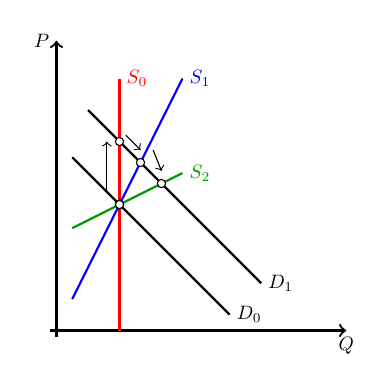
\begin{tikzpicture}[
					scale = 0.8,
					every node/.style = {scale = 0.7},
					declare function = {
						da(\x) = 3-\x;
						db(\x) = 4-\x;
						sa(\x) = 2*\x;
						sb(\x) = 1/2*\x+1.5;
					}
					]

					\draw[->,thick] (-0.1,0) -- (4.6,0)node[below]{$Q$};
					\draw[->,thick] (0,-0.1) -- (0,4.6)node[left]{$P$};

					\onslide<2->{
						\draw[thick,red] (1,0) -- (1,4)node[right]{$S_0$};
					}
					\onslide<3->{
						\draw[thick,domain=0.25:2.75,variable=\x] plot (\x,{da(\x)}) node[right]{$D_0$};
						\draw(1,{da(1)}) node[circle,fill=white,draw,solid,inner sep=1.5]{};

					}
					\onslide<4->{
						\draw[thick,domain=0.5:3.25,variable=\x] plot (\x,{db(\x)}) node[right]{$D_1$};
						\draw(1,{db(1)}) node[circle,fill=white,draw,solid,inner sep=1.5]{};
						\draw[<-] (0.8,{db(1)}) -- (0.8,{da(1)+0.2});
					}

					\onslide<5->{
						\draw[thick,blue,domain=0.25:2,variable=\x] plot (\x,{sa(\x)})node[right]{$S_1$};
						\draw({4/3},{sa(4/3)}) node[circle,fill=white,draw,solid,inner sep=1.5]{};
						\draw(1,{da(1)}) node[circle,fill=white,draw,solid,inner sep=1.5]{};
						\draw[->] ({1+0.1},{db(1)+0.1}) -- ({4/3},{sa(4/3)+0.2});
					}

					\onslide<6->{
						\draw[thick,green!60!black,domain=0.25:2,variable=\x] plot (\x,{sb(\x)})node[right]{$S_2$};
						\draw({5/3},{sb(5/3)}) node[circle,fill=white,draw,solid,inner sep=1.5]{};
						\draw(1,{da(1)}) node[circle,fill=white,draw,solid,inner sep=1.5]{};
						\draw[->] ({4/3+0.2},{sa(4/3)+0.2}) -- ({5/3},{sb(5/3)+0.2});
					}

				\end{tikzpicture}
			\end{center}
		\end{column}
		\begin{column}{0.47\textwidth}
			{\scriptsize
			A curto prazo, uma expans\~ao da procura de viagens para um destino em que os avi\~oes est\~ao sempre cheios s\'o ter\'a um efeito de aumento de pre\c cos: apenas os consumidores com maior disponibilidade a pagar poder\~ao viajar... ao longo prazo, podem planear-se mais voos para satisfazer a procura, podendo o pre\c co descer.
			}
		\end{column}
	\end{columns}
\end{frame}

\begin{frame}
	\frametitle{Quadro resumo Elasticidades}
	\begin{center}
		\begin{tabular}{ccc}
		\rowcolor{red!20!white} \textbf{Elasticidade} & \textbf{Valor} & \textbf{Conclus\~ao}\\ \hline
		\rowcolor{red!10!white}& $>1$ & Procura \'e el\'astica \\
		\rowcolor{red!10!white}& $= 1$ & Procura tem elasticidade unit\'aria \\
		\rowcolor{red!10!white}\multirow{-3}{*}{$|\varepsilon_D|$}& $< 1$ & Procura \'e inel\'astica \\ \hline
		\rowcolor{red!20!white}& $> 0$ & Bens substitutos\\
		\rowcolor{red!20!white}& $= 0$ & Bens independentes \\
		\rowcolor{red!20!white}\multirow{-3}{*}{$|\varepsilon_{x,y}|$}& $> 0$ & Bens complementares \\ \hline
		\rowcolor{red!10!white}& $< 0$ & Bem inferior \\
		\rowcolor{red!10!white}& $0<\eta<1$ & Bem normal \\
		\rowcolor{red!10!white}\multirow{-3}{*}{$\eta$}& $> 1$ & Bem de luxo \\\hline
		\rowcolor{red!20!white}& $> 1$ & Oferta \'e el\'astica\\
		\rowcolor{red!20!white}& $= 1$ & Oferta tem elasticidade unit\'aria \\
		\rowcolor{red!20!white}\multirow{-3}{*}{$\varepsilon_S$}& $< 1$ & Oferta \'e inel\'astica
		\end{tabular}
	\end{center}
\end{frame}
\section{Impostos}
\begin{frame}
	\frametitle{Impostos Indirectos}
	\begin{itemize}
		\setlength{\itemsep}{0.2cm}
		\item \textbf{Espec\'ificos:} O Governo cobra aos produtores uma certa import\^ancia fixa por cada unidade oferecida e vendida:
		\begin{itemize}
			\item Imposto sobre Ve\'iculos (ISV)
			\item Imposto sobre os Combust\'iveis (ISP)
		\end{itemize}
		\item \textbf{ad valorem:} o Governo cobra um valor que corresponde a uma percentagem aplicada ao pre\c co do produto:
		\begin{itemize}
			\item Imposto sobre o Valor Acrescentado (IVA)
		\end{itemize}
	\end{itemize}

\end{frame}

\begin{frame}
	\frametitle{Impostos Indirectos}
	\begin{itemize}
		\item O la\c camento de um imposto faz com que o pre\c co que o consumidor paga seja diferente do pre\c co que o produtor recebe numa transac\c c\~ao, ou seja: \[P_d=P_s+imposto\]
		\item Aos olhos do consumidor, a oferta apresentar-se-\`a distorcida, porque pagar\'a cada unidade mais cara...
	\end{itemize}
	\begin{center}
		Normalmente, \'e o produtor que tem a responsabilidade de cobrar o imposto e entregar o valor ao Estado (incid\^encia legal do imposto), mas veremos que o imposto tem incid\^encia econ\'omica em ambos os lados do mercado.
	\end{center}
\end{frame}

\begin{frame}
	\frametitle{Impostos Indirectos}
	O equil\'ibrio de mercado ap\'os introdu\c c\~ao do imposto \'e sempre caraterizado por:
	\begin{align*}	
		\left\{
		\begin{array}{c}
			Q_D=f_d(P_d)\\
			Q_S=f_s(P_S)\\
			Q_D=Q_S
			\\P_d=P_s+I
		\end{array}\right.
	\end{align*}
	No caso de um imposto espec\'ifico, $I$ \'e uma constante; no caso de um imposto \emph{ad valorem} \`a taxa $t$, tem-se: \[I=t\times P_S\]
\end{frame}

\begin{frame}
	\frametitle{Exemplo: \(Q_D=100-P\), \(Q_S=3P\)}

	Equil\'ibrio de Mercado, sem interven\c c\~oes

	\begin{align*}
		\left\{
			\begin{array}{c}
				Q_D=100-P\\
				Q_S=3P\\
				Q_D=Q_S
			\end{array}
		\right.
		\Leftrightarrow
		\left\{
			\begin{array}{c}
				Q_D=Q_S=75\\
				P=25
			\end{array}
		\right.
	\end{align*}

	\begin{center}
		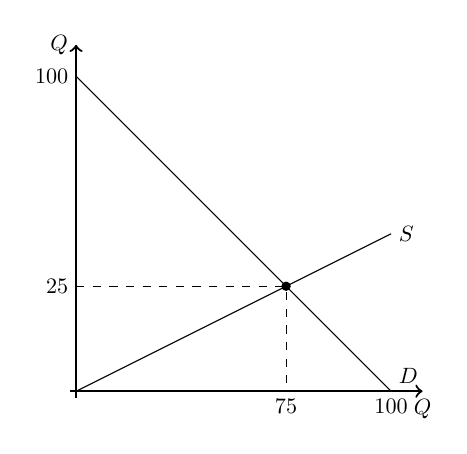
\begin{tikzpicture}[
			scale = 0.8,
			every node/.style = {scale = 0.8},
			declare function = {
				d(\x) = 5-\x;
				s(\x) = (1/2)*\x;
			}]

			\draw[->,thick] (-0.1,0) -- (5.5,0)node[below]{$Q$};
			\draw[->,thick] (0,-0.1) -- (0,5.5)node[left]{$Q$};

			\draw[domain=0:5,variable=\x] plot (\x,{d(\x)})node[above right]{$D$}node[below]{100};
			\draw[domain=0:5,variable=\x] plot (\x,{s(\x)})node[right]{$S$};

			\draw(0,{d(0)}) node[left]{100};

			\draw[dashed] (0,{5/3})node[left]{25} -- ({10/3},{5/3})node[circle,fill,inner sep=1.5]{} -- ({10/3},0)node[below]{75};

		\end{tikzpicture}
	\end{center}

\end{frame}

\begin{frame}
	\frametitle{Exemplo: \(Q_D=100-P\), \(Q_S=3P\)}
		Com lan\c camento de imposto espec\'ifico de 10um.
		\begin{align*}
			\left\{
				\begin{array}{c}
					Q_D=100-P_D\\
					Q_S=3P_S\\
					Q_D=Q_S\\
					P_D=P_S+10
				\end{array}
			\right.
			\Leftrightarrow
			\left\{
				\begin{array}{c}
					Q_D=Q_S=67.5\\
					P_D=32.5\\
					P_S=22.5
				\end{array}
			\right.
		\end{align*}

	\begin{center}
		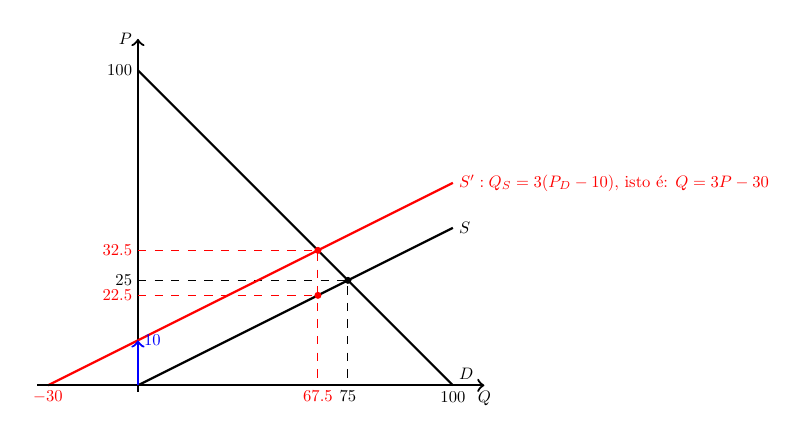
\begin{tikzpicture}[
			scale = 0.8,
			every node/.style = {scale = 0.6},
			declare function = {
				d(\x) = 5-\x;
				s(\x) = (1/2)*\x;
			}]

			\draw[->,thick] (-0.1,0) -- (5.5,0)node[below]{$Q$};
			\draw[->,thick] (0,-0.1) -- (0,5.5)node[left]{$P$};

			\draw[domain=0:5,variable=\x,thick] plot (\x,{d(\x)})node[above right]{$D$}node[below]{100};
			\draw[domain=0:5,variable=\x,thick] plot (\x,{s(\x)})node[right]{$S$};

			\draw(0,{d(0)}) node[left]{100};

			\draw[dashed] (0,{5/3})node[left]{25} -- ({10/3},{5/3})node[circle,fill,inner sep=1.5]{} -- ({10/3},0)node[below]{75};

			\onslide<2->{
				\draw[dashed,red] (0,{d(10/3.5)})node[left]{32.5} -- ({10/3.5},{d(10/3.5)}) node[circle,fill=red,inner sep=1.5]{} -- ({10/3.5},0)node[below]{67.5};
				\draw[dashed,red] (0,{s(10/3.5)})node[left]{22.5} -- ({10/3.5},{s(10/3.5)}) node[circle,fill=red,inner sep=1.5]{};
			}

			\onslide<3->{
				\draw[domain=0:5,variable=\x,thick,red] plot (\x,{s(\x)+(d(10/3.5)-s(10/3.5))}) node[right]{$S':Q_S=3(P_D-10)$, isto \'e: $Q=3P-30$};
			}

			\onslide<4->{
				\draw[domain={-2*(d(10/3.5)-s(10/3.5))}:0,variable=\x,thick,red] plot (\x,{s(\x)+(d(10/3.5)-s(10/3.5))});
				\draw[thick] (-1.6,0) -- (-0.1,0);
				\draw[red]({-2*(d(10/3.5)-s(10/3.5))},0)node[below]{$-30$};
			}

			\onslide<5->{
				\draw[thick,->,blue] (0,0) -- (0,{(d(10/3.5)-s(10/3.5))})node[right]{10};
			}

		\end{tikzpicture}
	\end{center}

\end{frame}

\begin{frame}
	\frametitle{Observa\c c\~oes:}
	\begin{itemize}
		\item A oferta n\~ao sofreu uma contrac\c c\~ao $S\parallel S'$!
		\item<2-> A oferta $S'$ \'e aquela que \'e vista pelo consumidor, j\'a que estamos a admitir que o imposto \'e recolhido e entregue ao Estado pelo produtor (incid\^encia legal do imposto)
		\item<3-> A oferta $S'$, aos olhos do consumidor, encontra-se distorcida face \`a oferta de mercado, que continua a ser $S$
		\item <4-> Os impostos indiretos s\~ao DISTORCION\'ARIOS
	\end{itemize}
\end{frame}

\begin{frame}
	\frametitle{Impostos Indirectos (imposto espec\'ifico)}
	\begin{center}
		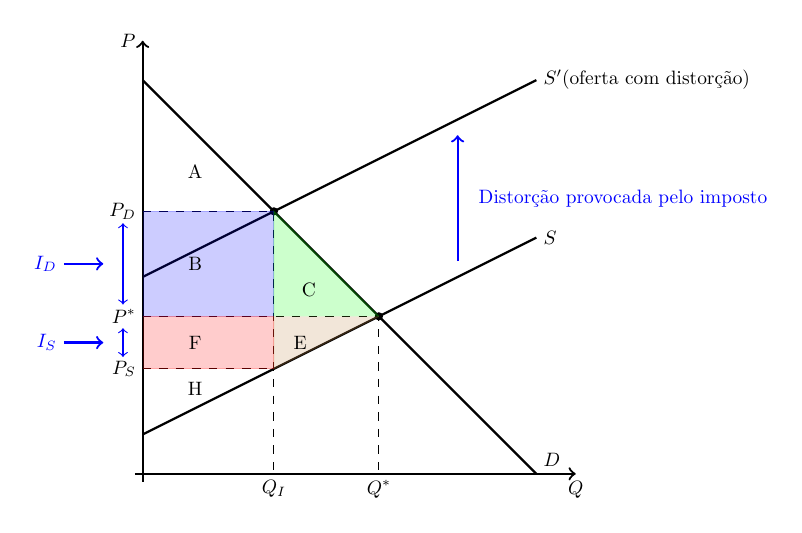
\begin{tikzpicture}[
			scale = 1,
			every node/.style = {scale = 0.7},
			declare function = {
				sa(\x) = 1/2 + 1/2 * \x;
				sb(\x) = 5/2 + 1/2 * \x;
				d(\x) = 5 - \x;
			}]

			\def\eqa{3}
			\def\eqb{5/3}

			\draw[->,thick] (-0.1,0) -- (5.5,0)node[below]{$Q$};
			\draw[->,thick] (0,-0.1) -- (0,5.5)node[left]{$P$};

			\draw[thick,domain=0:5,variable=\x] plot (\x,{d(\x)})node[above right]{$D$};
			\draw[thick,domain=0:5,variable=\x] plot (\x,{sa(\x)})node[right]{$S$};

			\onslide<2->{
				\draw[->,thick,blue] ({\eqa+1},{sa(\eqa+1)+0.2}) -- ({\eqa+1},{sb(\eqa+1)-0.2}) node[midway,xshift=3cm]{Distor\c c\~ao provocada pelo imposto};
				\draw[thick,domain=0:5,variable=\x] plot (\x,{sb(\x)})node[right]{$S'$(oferta com distor\c c\~ao)};
			}

			\onslide<3->{
				\draw[dashed] (0,{sa(\eqa)})node[left]{$P^*$} -- (\eqa,{sa(\eqa)})node[circle,fill,inner sep=1.5]{} -- (\eqa,0)node[below]{$Q^*$};
			}

			\onslide<4->{
				\draw[dashed] (0,{sb(\eqb)})node[left]{$P_D$} -- (\eqb,{sb(\eqb)})node[circle,fill,inner sep=1.5]{} -- (\eqb,0)node[below]{$Q_I$};
				\draw[dashed] (0,{sa(\eqb)})node[left]{$P_S$} -- (\eqb,{sa(\eqb)});
			}

			\onslide<5->{
				\draw[fill,opacity=0.2,blue] (0,{sa(\eqa)}) -- (\eqb,{sa(\eqa)}) -- (\eqb,{sb(\eqb)}) -- (0,{sb(\eqb)});
				\draw[fill,opacity=0.2,red] (0,{sa(\eqa)}) -- (\eqb,{sa(\eqa)}) -- (\eqb,{sa(\eqb)}) -- (0,{sa(\eqb)});
				\draw[fill,opacity=0.2,brown] (\eqb,{sa(\eqa)}) -- (\eqb,{sa(\eqb)}) -- (\eqa,{sa(\eqa)});
				\draw[fill,opacity=0.2,green] (\eqb,{sa(\eqa)}) -- (\eqb,{sb(\eqb)}) -- (\eqa,{sa(\eqa)});

				\draw({2/3},{(sb(\eqb)+d(2/3))/2})node[]{A};
				\draw({2/3},{(sa(2/3)+sa(\eqb))/2})node[]{H};
				\draw({2/3},{(sb(\eqb)+sa(\eqa))/2})node[]{B};
				\draw({2/3},{(sa(\eqb)+sa(\eqa))/2})node[]{F};
				\draw({\eqb+(\eqa-\eqb)/3},{(d((\eqa+\eqb)/2))+d(\eqa))/2})node[]{C};
				\draw({\eqb+(\eqa-\eqb)/4},{(sa(\eqb)+d(\eqa))/2})node[]{E};
			}

			\onslide<6->{
				\draw[thick,blue,->] (-1,{(sb(\eqb)+sa(\eqa))/2})node[left]{$I_D$} -- (-0.5,{(sb(\eqb)+sa(\eqa))/2});
				\draw[thick,blue,->] (-1,{(sa(\eqb)+sa(\eqa))/2})node[left]{$I_S$} -- (-0.5,{(sa(\eqb)+sa(\eqa))/2});
				\draw[<->,blue] (-0.25,{sa(\eqb)+0.15}) -- (-0.25,{sa(\eqa)-0.15});
				\draw[<->,blue] (-0.25,{sa(\eqa)+0.15}) -- (-0.25,{sb(\eqb)-0.15});
			}

		\end{tikzpicture}
	\end{center}
\end{frame}

\begin{frame}
	\frametitle{Em resumo...}
	\begin{center}
		{\renewcommand{\arraystretch}{1.5}
		\begin{tabular}{ccc}
			\rowcolor{iscal_color!50!white}& {\color{white}\textbf{Ap\'os imposto}} & {\color{white}\textbf{ Antes de imposto}} \\\hline
			\rowcolor{iscal_color!20!white}Excedente de Consumidor & $A$ & $A+B+C$ \\
			\rowcolor{iscal_color!10!white}Excedente de Produtor & $H$ & $F+E+H$ \\
			\rowcolor{iscal_color!20!white}Receita Fiscal (do Estado) & $B+F$ & -- \\
			\rowcolor{iscal_color!10!white}Perda Pura de Excedente & $C+E$ & -- \\
			\rowcolor{iscal_color!20!white}Quantidade Transaccionada & $Q_I$ & $Q^*$ \\
			\rowcolor{iscal_color!10!white}Pre\c co Transac\c c\~ao & $P_D$ ; $P_S$ & $P^*$
		\end{tabular}
		}
		\vskip 0.5cm
		Incid\^encia Econ\'omica do Imposto, por unidade transaccionada:\par $I_S$(produtor); $I_D$(consumidor)
	\end{center}
\end{frame}

\begin{frame}
	\frametitle{Em resumo no exemplo}
	\begin{columns}
		\begin{column}{0.5\textwidth}
			\begin{center}
				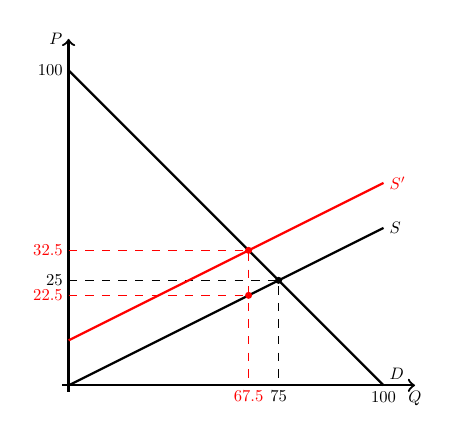
\begin{tikzpicture}[
					scale = 0.8,
					every node/.style = {scale = 0.6},
					declare function = {
						d(\x) = 5-\x;
						s(\x) = (1/2)*\x;
					}]

					\draw[->,thick] (-0.1,0) -- (5.5,0)node[below]{$Q$};
					\draw[->,thick] (0,-0.1) -- (0,5.5)node[left]{$P$};

					\draw[domain=0:5,variable=\x,thick] plot (\x,{d(\x)})node[above right]{$D$}node[below]{100};
					\draw[domain=0:5,variable=\x,thick] plot (\x,{s(\x)})node[right]{$S$};

					\draw(0,{d(0)}) node[left]{100};

					\draw[dashed] (0,{5/3})node[left]{25} -- ({10/3},{5/3})node[circle,fill,inner sep=1.5]{} -- ({10/3},0)node[below]{75};

					\draw[dashed,red] (0,{d(10/3.5)})node[left]{32.5} -- ({10/3.5},{d(10/3.5)}) node[circle,fill=red,inner sep=1.5]{} -- ({10/3.5},0)node[below]{67.5};
					\draw[dashed,red] (0,{s(10/3.5)})node[left]{22.5} -- ({10/3.5},{s(10/3.5)}) node[circle,fill=red,inner sep=1.5]{};

					\draw[domain=0:5,variable=\x,thick,red] plot (\x,{s(\x)+(d(10/3.5)-s(10/3.5))}) node[right]{$S'$};

				\end{tikzpicture}
			\end{center}
		\end{column}
		\begin{column}{0.4\textwidth}
			\(I_S=25-22.5=2.5um\)
			\(I_D=32.5-25=7.5um\)
			\(Total=10um=I\)
		\end{column}
	\end{columns}
\end{frame}

\begin{frame}
	\frametitle{Incid\^encia Econ\'omica}
	Quanto maior a elasticidade da procura (em m\'odulo) relativamente \`a da oferta, maior a incid\^encia do imposto sobre o lado da oferta.\par
	Pode demonstrar-se que:\[\frac{|\varepsilon_D|}{\varepsilon_S}=\frac{I_S}{I_D}\]
\end{frame}

\begin{frame}
	\frametitle{No exemplo}
		\begin{align*}
			Q_D=100-P&\rightarrow|\varepsilon_D|=\left|-1\times\frac{25}{75}\right| = 0.33\\
			Q_S=3P&\rightarrow\varepsilon_S=3\times\frac{25}{75}=1\\
			&\Downarrow\\
			\frac{|\varepsilon_D|}{\varepsilon_S}&=0.33\\
			\frac{I_S}{I_D}&=\frac{2.5}{7.5}=0.33
		\end{align*}
\end{frame}

\begin{frame}
	\frametitle{Elasticidade e Incid\^encia}
	\begin{align*}
		\frac{|\varepsilon_D|}{\varepsilon_S}&=\frac{I_S}{I_D}\\
		|\varepsilon_D|<\varepsilon_S\ &\Rightarrow\ I_D>I_S
	\end{align*}
\end{frame}

\begin{frame}
	\frametitle{Elasticidade e Incid\^encia}
	Quanto maior a elasticidade da procura (em m\'odulo) relativamente \`a da oferta, maior ser\'a a distor\c c\~ao da quantidade transacionada induzida pelo imposto (e, portanto, maior a perda de excedente econ\'omico).
\end{frame}

\begin{frame}
	\frametitle{Impostos Indirectos}
	A perda excedente econ\'omico (perda pura) \'e tanto menor quanto menor a elasticidade de um dos lados do mercado e, portanto, menor a dist\^ancia entre $Q^*$ e $Q_I$
	\begin{center}
		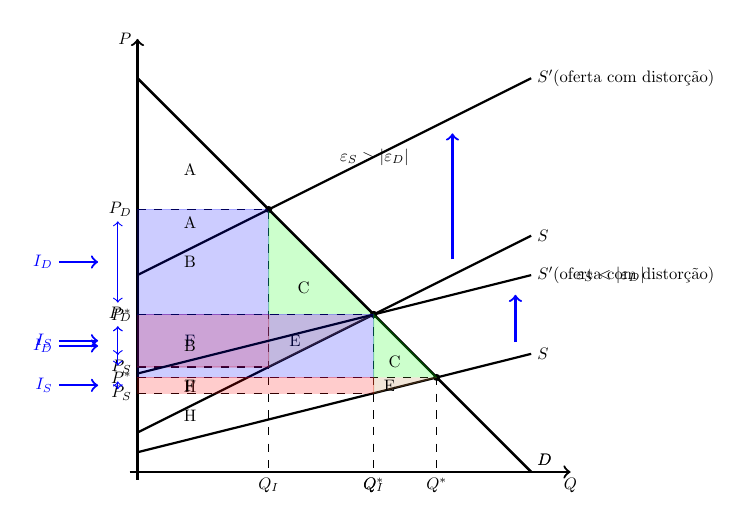
\begin{tikzpicture}[
			scale = 1,
			every node/.style = {scale = 0.6},
			declare function = {
				sa(\x) = 1/2 + 1/2 * \x;
				sb(\x) = 5/2 + 1/2 * \x;
				sc(\x) = 1/4 + 1/4 * \x;
				sd(\x) = 5/4 + 1/4 * \x;
				d(\x) = 5 - \x;
			}]

			\def\eqa{3}
			\def\eqb{5/3}
			\def\eqc{19/5}
			\def\eqd{3}

			\draw[->,thick] (-0.1,0) -- (5.5,0)node[below]{$Q$};
			\draw[->,thick] (0,-0.1) -- (0,5.5)node[left]{$P$};

			\onslide<1>{

				\draw[thick,domain=0:5,variable=\x] plot (\x,{d(\x)})node[above right]{$D$};
				\draw[thick,domain=0:5,variable=\x] plot (\x,{sa(\x)})node[right]{$S$};

				\draw[->,thick,blue] ({\eqa+1},{sa(\eqa+1)+0.2}) -- ({\eqa+1},{sb(\eqa+1)-0.2}) node[midway,xshift=3cm]{};
				\draw[thick,domain=0:5,variable=\x] plot (\x,{sb(\x)})node[right]{$S'$(oferta com distor\c c\~ao)};

				\draw[dashed] (0,{sa(\eqa)})node[left]{$P^*$} -- (\eqa,{sa(\eqa)})node[circle,fill,inner sep=1.5]{} -- (\eqa,0)node[below]{$Q^*$};

				\draw[dashed] (0,{sb(\eqb)})node[left]{$P_D$} -- (\eqb,{sb(\eqb)})node[circle,fill,inner sep=1.5]{} -- (\eqb,0)node[below]{$Q_I$};
				\draw[dashed] (0,{sa(\eqb)})node[left]{$P_S$} -- (\eqb,{sa(\eqb)});

				\draw[fill,opacity=0.2,blue] (0,{sa(\eqa)}) -- (\eqb,{sa(\eqa)}) -- (\eqb,{sb(\eqb)}) -- (0,{sb(\eqb)});
				\draw[fill,opacity=0.2,red] (0,{sa(\eqa)}) -- (\eqb,{sa(\eqa)}) -- (\eqb,{sa(\eqb)}) -- (0,{sa(\eqb)});
				\draw[fill,opacity=0.2,brown] (\eqb,{sa(\eqa)}) -- (\eqb,{sa(\eqb)}) -- (\eqa,{sa(\eqa)});
				\draw[fill,opacity=0.2,green] (\eqb,{sa(\eqa)}) -- (\eqb,{sb(\eqb)}) -- (\eqa,{sa(\eqa)});

				\draw({2/3},{(sb(\eqb)+d(2/3))/2})node[]{A};
				\draw({2/3},{(sa(2/3)+sa(\eqb))/2})node[]{H};
				\draw({2/3},{(sb(\eqb)+sa(\eqa))/2})node[]{B};
				\draw({2/3},{(sa(\eqb)+sa(\eqa))/2})node[]{F};
				\draw({\eqb+(\eqa-\eqb)/3},{(d((\eqa+\eqb)/2))+d(\eqa))/2})node[]{C};
				\draw({\eqb+(\eqa-\eqb)/4},{(sa(\eqb)+d(\eqa))/2})node[]{E};

				\draw[thick,blue,->] (-1,{(sb(\eqb)+sa(\eqa))/2})node[left]{$I_D$} -- (-0.5,{(sb(\eqb)+sa(\eqa))/2});
				\draw[thick,blue,->] (-1,{(sa(\eqb)+sa(\eqa))/2})node[left]{$I_S$} -- (-0.5,{(sa(\eqb)+sa(\eqa))/2});
				\draw[<->,blue] (-0.25,{sa(\eqb)+0.15}) -- (-0.25,{sa(\eqa)-0.15});
				\draw[<->,blue] (-0.25,{sa(\eqa)+0.15}) -- (-0.25,{sb(\eqb)-0.15});

				\draw(5.5,2.5)node[right]{\(\varepsilon_S<|\varepsilon_D|\)};

			}

			\onslide<2>{

				\draw[thick,domain=0:5,variable=\x] plot (\x,{d(\x)})node[above right]{$D$};
				\draw[thick,domain=0:5,variable=\x] plot (\x,{sc(\x)})node[right]{$S$};

				\draw[->,thick,blue] ({\eqc+1},{sc(\eqc+1)+0.2}) -- ({\eqc+1},{sd(\eqc+1)-0.2}) node[midway,xshift=3cm]{};
				\draw[thick,domain=0:5,variable=\x] plot (\x,{sd(\x)})node[right]{$S'$(oferta com distor\c c\~ao)};

				\draw[dashed] (0,{sc(\eqc)})node[left]{$P^*$} -- (\eqc,{sc(\eqc)})node[circle,fill,inner sep=1.5]{} -- (\eqc,0)node[below]{$Q^*$};

				\draw[dashed] (0,{sd(\eqd)})node[left]{$P_D$} -- (\eqd,{sd(\eqd)})node[circle,fill,inner sep=1.5]{} -- (\eqd,0)node[below]{$Q_I$};
				\draw[dashed] (0,{sc(\eqd)})node[left]{$P_S$} -- (\eqd,{sc(\eqd)});

				\draw[fill,opacity=0.2,blue] (0,{sc(\eqc)}) -- (\eqd,{sc(\eqc)}) -- (\eqd,{sd(\eqd)}) -- (0,{sd(\eqd)});
				\draw[fill,opacity=0.2,red] (0,{sc(\eqc)}) -- (\eqd,{sc(\eqc)}) -- (\eqd,{sc(\eqd)}) -- (0,{sc(\eqd)});
				\draw[fill,opacity=0.2,brown] (\eqd,{sc(\eqc)}) -- (\eqd,{sc(\eqd)}) -- (\eqc,{sc(\eqc)});
				\draw[fill,opacity=0.2,green] (\eqd,{sc(\eqc)}) -- (\eqd,{sd(\eqd)}) -- (\eqc,{sc(\eqc)});

				\draw({2/3},{(sd(\eqd)+d(2/3))/2})node[]{A};
				\draw({2/3},{(sc(2/3)+sc(\eqd))/2})node[]{H};
				\draw({2/3},{(sd(\eqd)+sc(\eqc))/2})node[]{B};
				\draw({2/3},{(sc(\eqd)+sc(\eqc))/2})node[]{F};
				\draw({\eqd+(\eqc-\eqd)/3},{(d((\eqc+\eqd)/2))+d(\eqc))/2})node[]{C};
				\draw({\eqd+(\eqc-\eqd)/4},{(sc(\eqd)+d(\eqc))/2})node[]{E};

				\draw[thick,blue,->] (-1,{(sd(\eqd)+sc(\eqc))/2})node[left]{$I_D$} -- (-0.5,{(sd(\eqd)+sc(\eqc))/2});
				\draw[thick,blue,->] (-1,{(sc(\eqd)+sc(\eqc))/2})node[left]{$I_S$} -- (-0.5,{(sc(\eqd)+sc(\eqc))/2});
				\draw[<->,blue] (-0.25,{sc(\eqd)+0.15}) -- (-0.25,{sc(\eqc)-0.15});
				\draw[<->,blue] (-0.25,{sc(\eqc)+0.15}) -- (-0.25,{sd(\eqd)-0.15});

				\draw(2.5,4)node [right]{\(\varepsilon_S>|\varepsilon_D|\)};

			}

		\end{tikzpicture}
	\end{center}
\end{frame}

\begin{frame}
	\frametitle{Impostos Indirectos}
	Um imposto indireto sem distor\c c\~oes (e portanto sem perda pura) s\'o \'e poss\'ivel se um dos lados do mercado tiver elasticidade nula...
		\begin{center}
		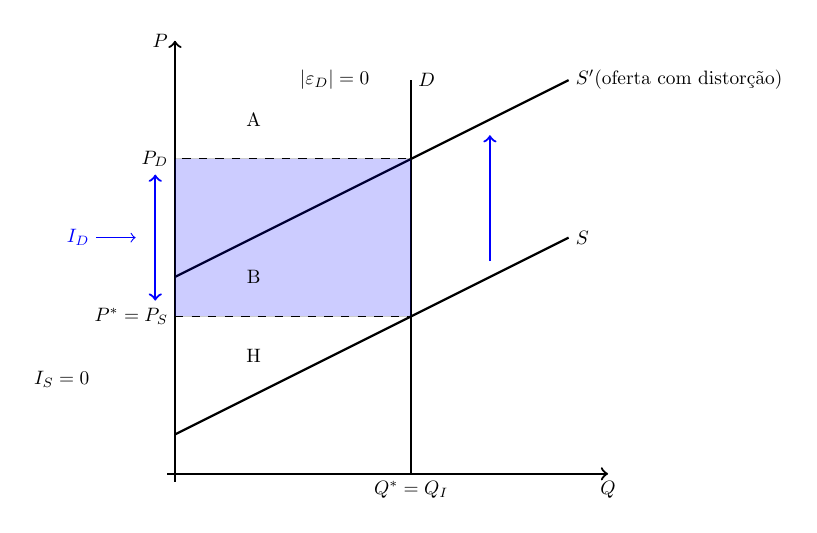
\begin{tikzpicture}[
			scale = 1,
			every node/.style = {scale = 0.7},
			declare function = {
				sa(\x) = 1/2 + 1/2 * \x;
				sb(\x) = 5/2 + 1/2 * \x;
				sc(\x) = 1/4 + 1/4 * \x;
				sd(\x) = 5/4 + 1/4 * \x;
			}]
			\def\eqa{3}
			\def\eqb{3}
			\def\eqc{3}
			\def\eqd{3}

			\draw[->,thick] (-0.1,0) -- (5.5,0)node[below]{$Q$};
			\draw[->,thick] (0,-0.1) -- (0,5.5)node[left]{$P$};

			\draw[thick] (3,0) node[below]{$Q^*=Q_I$} -- (3,5) node[right]{$D$};
			\draw[thick,domain=0:5,variable=\x] plot (\x,{sa(\x)})node[right]{$S$};

			\draw[->,thick,blue] ({\eqa+1},{sa(\eqa+1)+0.2}) -- ({\eqa+1},{sb(\eqa+1)-0.2}) node[midway,xshift=3cm]{};
			\draw[thick,domain=0:5,variable=\x] plot (\x,{sb(\x)})node[right]{$S'$(oferta com distor\c c\~ao)};

			\draw[dashed] (0,{sa(3)})node[left]{$P^*=P_S$} -- (3,{sa(3)}) -- (3,{sb(3)}) -- (0,{sb(3)})node[left]{$P_D$};
			\draw[fill=blue,opacity=0.2] (0,{sa(3)}) -- (3,{sa(3)}) -- (3,{sb(3)}) -- (0,{sb(3)});

			\draw(1.5,5)node[right]{\(|\varepsilon_D|=0\)};

			\draw[<->,blue,thick] (-0.25,{sa(3)+0.2}) -- (-0.25,{sb(3)-0.2});
			\draw[->,blue] (-1,{(sa(3)+sb(3))/2}) node[left]{$I_D$} -- (-0.5,{(sa(3)+sb(3))/2});
			\draw (-1,{(sa(3)+sb(3))/5}) node[left]{$I_S=0$};

			\draw(1,1.5)node[]{H};
			\draw(1,2.5)node[]{B};
			\draw(1,4.5)node[]{A};

		\end{tikzpicture}
	\end{center}
\end{frame}

\begin{frame}
	\frametitle{Impostos Indirectos}
	Com lan\c camento de imposto \emph{ad valorem} a 30\%
	\begin{align*}
		\left\{
			\begin{array}{c}
				Q_D=100-P_D\\
				Q_S=3P_S\\
				Q_D=Q_S\\
				P_D=P_S+0.3P_S
			\end{array}
		\right.
		\Leftrightarrow
		\left\{
			\begin{array}{c}
				Q_D=Q_S=69.77\\
				P_D=30.233\\
				P_S=23.256
			\end{array}
		\right.
	\end{align*}

	\begin{center}
		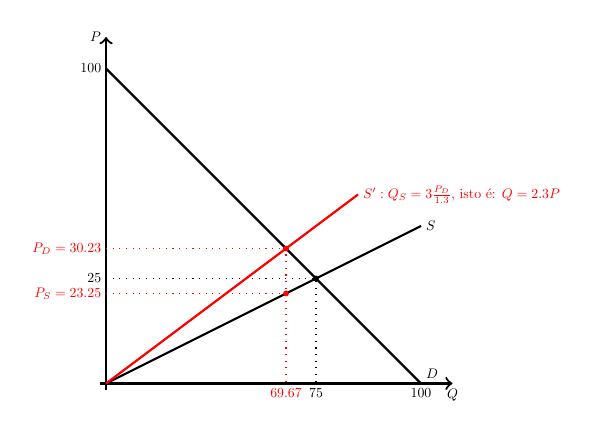
\begin{tikzpicture}[
			scale = 0.8,
			every node/.style = {scale = 0.5},
			declare function = {
				d(\x) = 5-\x;
				s(\x) = (1/2)*\x;
			}]

			\draw[->,thick] (-0.1,0) -- (5.5,0)node[below]{$Q$};
			\draw[->,thick] (0,-0.1) -- (0,5.5)node[left]{$P$};

			\draw[domain=0:5,variable=\x,thick] plot (\x,{d(\x)})node[above right]{$D$}node[below]{100};
			\draw[domain=0:5,variable=\x,thick] plot (\x,{s(\x)})node[right]{$S$};

			\draw(0,{d(0)}) node[left]{100};

			\draw[dotted] (0,{5/3})node[left]{25} -- ({10/3},{5/3})node[circle,fill,inner sep=1.5]{} -- ({10/3},0)node[below]{75};

			\draw[dotted,red] (0,{d(10/3.5)})node[left]{$P_D=30.23$} -- ({10/3.5},{d(10/3.5)}) node[circle,fill=red,inner sep=1.5]{} -- ({10/3.5},0)node[below]{69.67};
			\draw[dotted,red] (0,{s(10/3.5)})node[left]{$P_S=23.25$} -- ({10/3.5},{s(10/3.5)}) node[circle,fill=red,inner sep=1.5]{};

			\draw[domain=0:4,variable=\x,thick,red] plot (\x,{(d(10/3.5)/(10/3.5))*\x}) node[right]{$S':Q_S=3\frac{P_D}{1.3}$, isto \'e: $Q=2.3 P$};

		\end{tikzpicture}
	\end{center}

\end{frame}

\begin{frame}
	\frametitle{Impostos Indiretos (\emph{ad valorem} \`a taxa $t$)}
	\begin{center}
		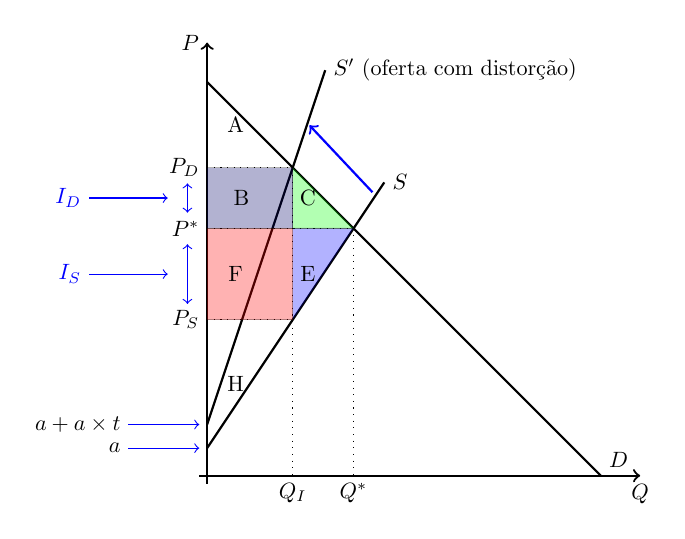
\begin{tikzpicture}[
			scale = 1,
			every node/.style = {scale = 0.8},
			declare function = {
				d(\x) = 5-\x;
				sa(\x) = 0.35+1.5*\x;
				sb(\x) = 0.65+3*\x;
				sc(\x) = 0.5+(1/2)*\x;
				sd(\x) = 0.5+(1/4)*\x;
			}]

			\def\eqa{93/50}
			\def\eqb{87/80}

			\draw[->,thick] (-0.1,0) -- (5.5,0)node[below]{$Q$};
			\draw[->,thick] (0,-0.1) -- (0,5.5)node[left]{$P$};

			\draw[domain=0:5,variable=\x,thick] plot (\x,{d(\x)})node[above right]{$D$}node[below]{};
			\draw[domain=0:2.25,variable=\x,thick] plot (\x,{sa(\x)})node[right]{$S$};
			\draw[domain=0:1.5,variable=\x,thick] plot (\x,{sb(\x)})node[right]{$S'$ (oferta com distor\c c\~ao)};
			\draw[blue,->] (-1,{sb(0)})node[text=black,left]{$a+a\times t$} -- (-0.1,{sb(0)});
			\draw[blue,->] (-1,{sa(0)})node[text=black,left]{$a$} -- (-0.1,{sa(0)});

			\draw[->,thick,blue] (2.1,{sa(2.1)+0.1}) -- (1.3,{sb(1.3)-0.1});

			\draw[dotted] (0,{sb(\eqb)})node[left]{$P_D$} -- (\eqb,{sb(\eqb)}) -- (\eqb,0)node[below]{$Q_I$};
			\draw[dotted] (0,{sa(\eqa)})node[left]{$P^*$} -- (\eqa,{sa(\eqa)}) -- (\eqa,0)node[below]{$Q^*$};
			\draw[dotted] (0,{sa(\eqb)})node[left]{$P_S$} -- (\eqb,{sa(\eqb)});

			\draw[blue,<->] (-0.25,{sa(\eqb)+0.2}) -- (-0.25,{sa(\eqa)-0.2});
			\draw[blue,<->] (-0.25,{sa(\eqa)+0.2}) -- (-0.25,{sb(\eqb)-0.2});
			\draw[blue,->] (-1.5,{(sa(\eqb)+sa(\eqa))/2})node[left]{$I_S$} -- (-0.5,{(sa(\eqb)+sa(\eqa))/2});
			\draw[blue,->] (-1.5,{(sa(\eqa)+sb(\eqb))/2})node[left]{$I_D$} -- (-0.5,{(sa(\eqa)+sb(\eqb))/2});

			\draw[fill=red,opacity=0.3] (0,{sa(\eqb)}) -- (\eqb,{sa(\eqb)}) -- (\eqb,{sa(\eqa)}) -- (0,{sa(\eqa)});
			\draw[fill=blue,opacity=0.3] (\eqb,{sa(\eqb)}) -- (\eqa,{sa(\eqa)}) -- (\eqb,{sa(\eqa)});
			\draw[fill=green,opacity=0.3] (\eqa,{sa(\eqa)}) -- (\eqb,{sa(\eqa)}) -- (\eqb,{sb(\eqb)});
			\draw[fill=blue!40!black,opacity=0.3] (0,{sa(\eqa)}) -- (\eqb,{sa(\eqa)}) -- (\eqb,{sb(\eqb)}) -- (0,{sb(\eqb)});

			\draw ({\eqb/3},{(sa(\eqb)+sa(\eqa))/2}) node[]{F};
			\draw ({\eqb/2.5},{(sb(\eqb)+sa(\eqa))/2}) node[]{B};
			\draw ({\eqb/3},{(sb(\eqb)+d(0))/2}) node[]{A};
			\draw ({\eqb/3},{(sa(\eqb)+sa(0))/2}) node[]{H};
			\draw ({\eqb+(\eqa-\eqb)/4},{(sa(\eqb)+sa(\eqa))/2}) node[]{E};
			\draw ({\eqb+(\eqa-\eqb)/4},{(sb(\eqb)+sa(\eqa))/2}) node[]{C};

		\end{tikzpicture}
	\end{center}
\end{frame}

\begin{frame}
	\frametitle{Subs\'idio espec\'ifico}
	Com lan\c camento de subs\'idio espec\'ifico de 10um:
	\begin{align*}
		\left\{
			\begin{array}{c}
				Q_D=100-P_D\\
				Q_S=3P_S\\
				Q_D=Q_S\\
				P_D=P_S-10
			\end{array}
		\right.
		\Leftrightarrow
		\left\{
			\begin{array}{c}
				Q_D=Q_S=82.5\\
				P_D=17.5\\
				P_S=27.5
			\end{array}
		\right.
	\end{align*}

	\begin{center}
		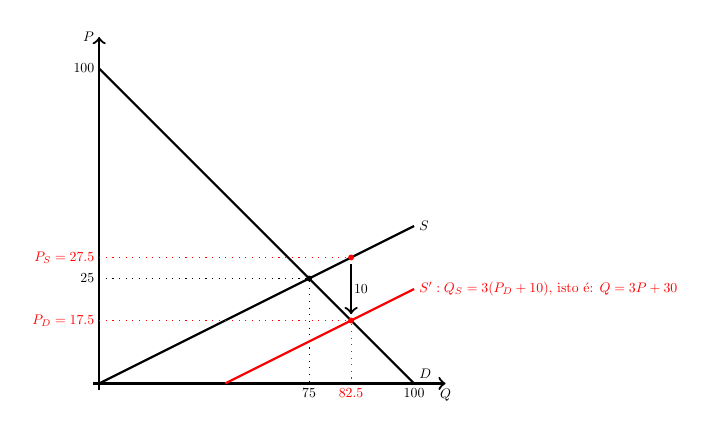
\begin{tikzpicture}[
			scale = 0.8,
			every node/.style = {scale = 0.5},
			declare function = {
				d(\x) = 5-\x;
				s(\x) = (1/2)*\x;
			}]

			\draw[->,thick] (-0.1,0) -- (5.5,0)node[below]{$Q$};
			\draw[->,thick] (0,-0.1) -- (0,5.5)node[left]{$P$};

			\draw[domain=0:5,variable=\x,thick] plot (\x,{d(\x)})node[above right]{$D$}node[below]{100};
			\draw[domain=0:5,variable=\x,thick] plot (\x,{s(\x)})node[right]{$S$};

			\draw(0,{d(0)}) node[left]{100};

			\draw[dotted] (0,{5/3})node[left]{25} -- ({10/3},{5/3})node[circle,fill,inner sep=1.5]{} -- ({10/3},0)node[below]{75};

			\onslide<2->{

				\draw[dotted,red] (0,{d(4)})node[left]{$P_D=17.5$} -- ({4},{d(4)}) node[circle,fill=red,inner sep=1.5]{};
				\draw[dotted,red] (0,{s(4)})node[left]{$P_S=27.5$} -- ({4},{s(4)}) node[circle,fill=red,inner sep=1.5]{} -- ({4},0)node[below]{82.5};

				\draw[domain=2:5,variable=\x,thick,red] plot (\x,{(s(\x-2)}) node[right]{$S':Q_S=3(P_D+10)$, isto \'e: $Q=3 P+30$};

			}

			\onslide<3->{
				\draw[->,thick] ({4},{s(4)-0.1}) -- ({4},{d(4)+0.1})node[midway,xshift=0.25cm]{$10$};
			}

		\end{tikzpicture}
	\end{center}
\end{frame}

\begin{frame}
	\frametitle{Subs\'idios}
	A perda excedente econ\'omico (perda pura, $C+E$), neste caso, \'e parte da despesa fiscal ($B+G+C+F+J+E$) que n\~ao \'e apropriada nem pelos consumidores (excedente $A+B+F+K$) nem pelos produtores (excedente $H+F+B+G$)
	\begin{center}
		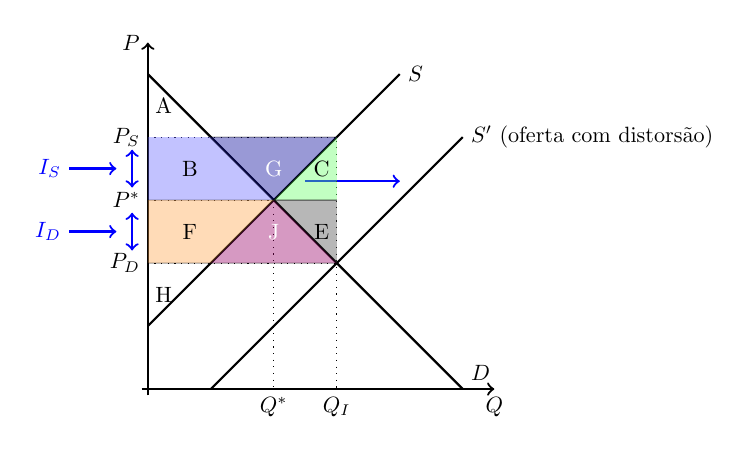
\begin{tikzpicture}[
			scale = 0.8,
			every node/.style = {scale = 0.8},
			declare function = {
				d(\x) = 5-\x;
				sa(\x) = 1+\x;
				sb(\x) = -1 + \x;
			}]

			\def\eqa{2}
			\def\eqb{3}

			\draw[->,thick] (-0.1,0) -- (5.5,0)node[below]{$Q$};
			\draw[->,thick] (0,-0.1) -- (0,5.5)node[left]{$P$};

			\draw[thick,domain=0:5,variable=\x] plot (\x,{d(\x)})node[above right]{$D$};
			\draw[thick,domain=0:4,variable=\x] plot (\x,{sa(\x)})node[right]{$S$};
			\draw[dotted] (0,{d(\eqa)})node[left]{$P^*$} -- (\eqa,{d(\eqa)}) -- (\eqa,0)node[below]{$Q^*$};

			\onslide<2>{
				\draw[->,blue,thick] ({\eqa+0.5},{sa(\eqa+0.3)}) -- ({\eqa+2},{sa(\eqa+0.3)});	
			}

			\onslide<2->{
				\draw[thick,domain=1:5,variable=\x] plot (\x,{sb(\x)})node[right]{$S'$ (oferta com distors\~ao)};	
			}

			\onslide<3->{
				\draw[dotted] (0,{sa(\eqb)})node[left]{$P_S$} -- (\eqb,{sa(\eqb)}) -- (\eqb,0)node[below]{$Q_I$};
				\draw[dotted] (0,{sb(\eqb)})node[left]{$P_D$} -- (\eqb,{sb(\eqb)});
			}

			\onslide<4->{
				\draw[blue,thick,<->] (-0.25,{sb(\eqb)+0.2}) -- (-0.25,{d(\eqa)-0.2});
				\draw[blue,thick,<->] (-0.25,{d(\eqa)+0.2}) -- (-0.25,{sa(\eqb)-0.2});
				\draw[blue,thick,->] (-1.25,{(sb(\eqb)+d(\eqa))/2})node[left]{$I_D$} -- (-0.5,{(sb(\eqb)+d(\eqa))/2});
				\draw[blue,thick,->] (-1.25,{(sa(\eqb)+d(\eqa))/2})node[left]{$I_S$} -- (-0.5,{(sa(\eqb)+d(\eqa))/2});
			}

			\onslide<5->{
				\draw[fill=blue!60!white,opacity=0.4] (0,{sa(\eqb)}) -- (0,{d(\eqa)}) -- (\eqa,{d(\eqa)}) -- (1,{sa(\eqb)});
				\draw[fill=blue!60!black,opacity=0.4] (1,{sa(\eqb)}) -- (\eqb,{sa(\eqb)}) -- (\eqa,{d(\eqa)});
				\draw[fill=green!60!white,opacity=0.4] (\eqb,{sa(\eqb)}) -- (\eqa,{d(\eqa)}) -- (\eqb,{sa(\eqa)});
				%\draw[fill=green!60!black,opacity=0.4] (\eqb,{sa(\eqa)}) -- (\eqa,{d(\eqa)}) -- (\eqb,{sb(\eqb)});
				\draw[fill=gray!60!black,opacity=0.4] (\eqb,{sa(\eqa)}) -- (\eqa,{d(\eqa)}) -- (\eqb,{sb(\eqb)});
				\draw[fill=red!60!blue,opacity=0.4] (\eqa,{d(\eqa)}) -- (\eqb,{sb(\eqb)}) -- (1,{sb(\eqb)});
				\draw[fill=orange!70!white,opacity=0.4] (\eqa,{sa(\eqa)}) -- (1,{sb(\eqb)}) -- (0,{sb(\eqb)}) -- (0,{sa(\eqa)});
			}

			\onslide<6->{
				\draw(0.25,{(d(0)+sa(\eqb))/2})node[]{A};
				\draw({\eqa/3},{(sa(\eqb)+sa(\eqa))/2})node[]{B};
				\draw({\eqa/3},{(sa(\eqa)+sb(\eqb))/2})node[]{F};
				\draw(0.25,{(sa(0)+sb(\eqb))/2})node[]{H};

				\draw[white](\eqa,{(d(1)+sa(\eqa))/2})node[]{G};
				\draw[white](\eqa,{(sa(1)+sa(\eqa))/2})node[]{J};
				
				\draw({\eqb*0.92},{(sa(\eqb)+sa(\eqa))/2})node[]{C};
				\draw({\eqb*0.92},{(sa(\eqa)+sb(\eqb))/2})node[]{E};
			}

		\end{tikzpicture}
	\end{center}
\end{frame}

\begin{frame}
	\frametitle{Em resumo}
	\begin{center}
		{
		\renewcommand{\arraystretch}{1.5}
		\footnotesize
		\begin{tabular}{ccc}
		\rowcolor{iscal_color}	& {\color{white}\textbf{Ap\'os subs\'idio}} & {\color{white}\textbf{Antes de subs\'idio}} \\
		\hline
		\rowcolor{iscal_color!10!white} Excedente de Consumidor 	& $A+B+F+J$ 	& $A+B$ \\
		\rowcolor{iscal_color!20!white} Excedente de Produtor 		& $F+H+B+G$ 	& $F+H$ \\
		\rowcolor{iscal_color!10!white} Despesa Fiscal (do Estado)  & $B+G+C+F+J+E$ & --\\
		\rowcolor{iscal_color!20!white} Perda Pura de Excedente 	& $C+E$ 		& -- \\
		\rowcolor{iscal_color!10!white} Quantidade Transacionada 	& $Q_I$ 		& $Q^*$ \\
		\rowcolor{iscal_color!20!white} Pre\c co Transac\c c\~ao 	& $P_D$; $P_S$  & $P^*$
		\end{tabular}

		\vspace{0.3cm}

		Incid\^encia Econ\'omica do subs\'idio, por unidade transacionada:\par $I_S(produtor)$; $I_D(consumidor)$
		}
	\end{center}
\end{frame}

\begin{frame}
	\frametitle{Em resumo}
	\begin{columns}
		\begin{column}{0.6\textwidth}
			\begin{center}
				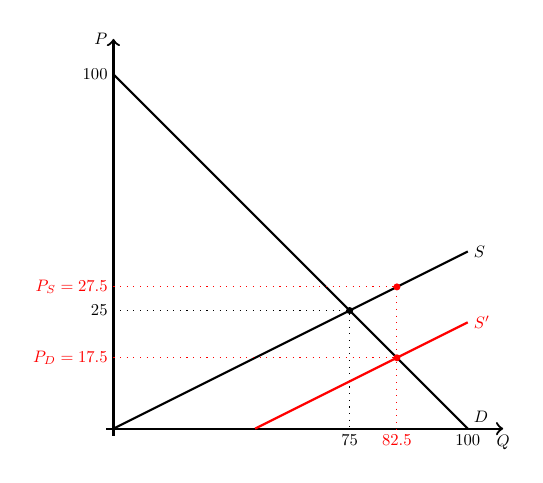
\begin{tikzpicture}[
					scale = 0.9,
					every node/.style = {scale = 0.6},
					declare function = {
						d(\x) = 5-\x;
						s(\x) = (1/2)*\x;
					}]

					\draw[->,thick] (-0.1,0) -- (5.5,0)node[below]{$Q$};
					\draw[->,thick] (0,-0.1) -- (0,5.5)node[left]{$P$};

					\draw[domain=0:5,variable=\x,thick] plot (\x,{d(\x)})node[above right]{$D$}node[below]{100};
					\draw[domain=0:5,variable=\x,thick] plot (\x,{s(\x)})node[right]{$S$};

					\draw(0,{d(0)}) node[left]{100};

					\draw[dotted] (0,{5/3})node[left]{25} -- ({10/3},{5/3})node[circle,fill,inner sep=1.5]{} -- ({10/3},0)node[below]{75};

					\draw[dotted,red] (0,{d(4)})node[left]{$P_D=17.5$} -- ({4},{d(4)}) node[circle,fill=red,inner sep=1.5]{};
					\draw[dotted,red] (0,{s(4)})node[left]{$P_S=27.5$} -- ({4},{s(4)}) node[circle,fill=red,inner sep=1.5]{} -- ({4},0)node[below]{82.5};

					\draw[domain=2:5,variable=\x,thick,red] plot (\x,{(s(\x-2)}) node[right]{$S'$};

				\end{tikzpicture}
			\end{center}
		\end{column}
		\begin{column}{0.4\textwidth}
			\begin{itemize}
				\item \(I_S=27.5-25=2.5um\)
				\item \(I_D=25-17.5=7.5um\)
				\item \(Total = 10um = I\)
			\end{itemize}
		\end{column}
	\end{columns}
\end{frame}
\section{Controlo de Pre\c cos}
\begin{frame}
	\frametitle{Controlo de pre\c cos: $P_{max}$}
	O Governo fixa compulsivamente um pre\c co abaixo do pre\c co de equil\'ibrio:

	\vspace{0.2cm}

	Pretende impedir que o pre\c co do bem suba acima do pre\c co tabelado, de modo a beneficiar os consumidores (ex.: controlo das rendas)
	
\end{frame}

\begin{frame}
	\frametitle{Pre\c cos M\'aximos}
	\begin{columns}
		\begin{column}{0.6\textwidth}
			\begin{center}
				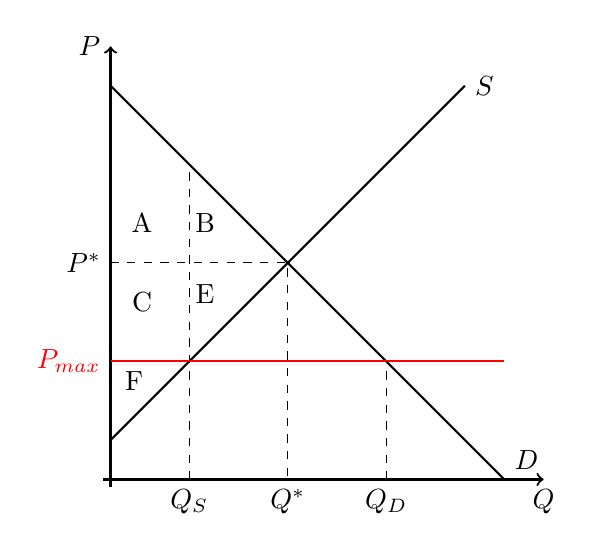
\begin{tikzpicture}[
					scale = 1,
					every node/.style = {scale = 1},
					declare function = {
						d(\x) = 5 - \x;
						s(\x) = 0.5 + \x;
					}]
					\def\eq{9/4}

					\draw[thick,->] (-0.1,0) -- (5.5,0)node[below]{$Q$};
					\draw[thick,->] (0,-0.1) -- (0,5.5)node[left]{$P$};

					\draw[thick,domain=0:5,variable=\x] plot (\x,{d(\x)})node[above right]{$D$};
					\draw[thick,domain=0:4.5,variable=\x] plot (\x,{s(\x)})node[right]{$S$};

					\draw[thick,red] (0,1.5)node[left]{$P_{max}$} -- (5,1.5);
					\draw[dashed] (0,{s(\eq)})node[left]{$P^*$} -- (\eq,{s(\eq)}) -- (\eq,0)node[below]{$Q^*$};

					\draw[dashed] (1,0)node[below]{$Q_S$} -- (1,{d(1)});
					\draw[dashed] (3.5,0)node[below]{$Q_D$} -- (3.5,{d(3.5)});

					\draw(0.4,{d(\eq)+0.5})node[]{A};
					\draw(0.4,{d(\eq)-0.5})node[]{C};
					\draw(0.3,{d(\eq)-1.5})node[]{F};
					\draw(1.2,{d(\eq)+0.5})node[]{B};
					\draw(1.2,{d(\eq)-0.4})node[]{E};

				\end{tikzpicture}
			\end{center}
		\end{column}
		\begin{column}{0.4\textwidth}
			\begin{itemize}
				\item O mercado fica equilibrado?
				\item Qual a altera\c c\~ao ao excedente do consumidor? Continua a ter o mesmo significado?
				\item Qual a altera\c c\~ao no excedente do produtor?
			\end{itemize}
		\end{column}
	\end{columns}
\end{frame}

\begin{frame}
	\frametitle{Pre\c cos M\'aximos: reflex\~ao}
	\begin{enumerate}
		\item Ser\~ao os consumidores que mais valorizam o bem aqueles que o conseguem consumir?
		\item Quais as consequ\^encias da possibilidade de revender o bem?
		\item Estar\~ao os produtores dispostos a apostar na qualidade, num mercado regulado desta maneira?
		\item Como se aplicam as conclus\~oes acima ao mercado imobili\'ario no caso de rendas controladas? (admitindo que n\~ao h\'a falhas de mercado e que a concorr\^encia perfeita \'e uma boa forma de o descrever?)
	\end{enumerate}
\end{frame}

\begin{frame}
	\frametitle{Controlo de Pre\c cos - $P_{min}$}
	O Governo fixa compulsivamente um pre\c co acima do pre\c co de equil\'ibrio
	\begin{itemize}
		\item estabelece um pre\c co limite para que os produtores possam vender o bem (ex.: pre\c co de alguns produtos agr\'icolas). O objectivo \'e, normalmente, beneficiar os produtores.
		\item O sal\'ario m\'inimo \'e um pre\c co m\'inimo estabelecido no mercado do trabalho.
	\end{itemize}
\end{frame}

\begin{frame}
	\frametitle{Pre\c cos M\'inimos}
	\begin{columns}
		\begin{column}{0.6\textwidth}
			\begin{center}
				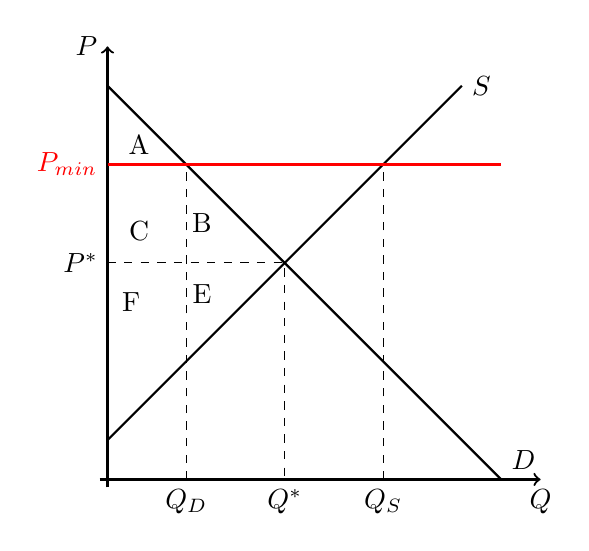
\begin{tikzpicture}[
					scale = 1,
					every node/.style = {scale = 1},
					declare function = {
						d(\x) = 5 - \x;
						s(\x) = 0.5 + \x;
					}]
					\def\eq{9/4}

					\draw[thick,->] (-0.1,0) -- (5.5,0)node[below]{$Q$};
					\draw[thick,->] (0,-0.1) -- (0,5.5)node[left]{$P$};

					\draw[thick,domain=0:5,variable=\x] plot (\x,{d(\x)})node[above right]{$D$};
					\draw[thick,domain=0:4.5,variable=\x] plot (\x,{s(\x)})node[right]{$S$};

					\draw[thick,red] (0,4)node[left]{$P_{min}$} -- (5,4);
					\draw[dashed] (0,{s(\eq)})node[left]{$P^*$} -- (\eq,{s(\eq)}) -- (\eq,0)node[below]{$Q^*$};

					\draw[dashed] (1,0)node[below]{$Q_D$} -- (1,{d(1)});
					\draw[dashed] (3.5,0)node[below]{$Q_S$} -- (3.5,{s(3.5)});

					\draw(0.4,{d(\eq)+1.5})node[]{A};
					\draw(0.4,{d(\eq)+0.4})node[]{C};
					\draw(0.3,{d(\eq)-0.5})node[]{F};
					\draw(1.2,{d(\eq)+0.5})node[]{B};
					\draw(1.2,{d(\eq)-0.4})node[]{E};

				\end{tikzpicture}
			\end{center}
		\end{column}
		\begin{column}{0.4\textwidth}
			\begin{itemize}
				\item O mercado fica equilibrado?
				\item Qual a altera\c c\~ao ao excedente do consumidor?
				\item Qual a altera\c c\~ao no excedente do produtor? Continua a ter o mesmo significado?
			\end{itemize}
		\end{column}
	\end{columns}
\end{frame}

\begin{frame}
	\frametitle{Pre\c cos M\'inimos: reflex\~ao}
	\begin{enumerate}
		\item Ser\~ao os consumidores que mais valorizam o bem aqueles que o conseguem consumir?
		\item Os produtores conseguem escoar todo o seu stock?
		\item O que poder\'a ser feito para evitar acumula\c c\~ao de stocks e manter o pre\c co alto?
		\item Haver\'a efici\^encia na utiliza\c c\~ao de recursos?
		\item Como se aplicam as conclus\~oes acima ao mercado do trabalho com o sal\'ario m\'inimo (admitindo que n\~ao h\'a falhas de mercado e que a concorr\^encia perfeita \'e uma boa forma de o descrever)
	\end{enumerate}
\end{frame}

\end{document}